% !TEX TS-program = pdflatex
% !TeX spellcheck = ru_RU
% !TEX root = main.tex


\documentclass[acmsmall, language=english, language=russian
  %, review
  %, xcolor
  %, hyperref={colorlinks=true}
  ]{acmart}

% !TEX TS-program = pdflatex
% !TeX spellcheck = en_US
% !TEX root = main.tex
\newcommand{\OCanren}{\textsc{OCanren}}
\newcommand{\OCaml}{\textsc{OCaml}}
\newcommand{\Scheme}{\textsc{Scheme}}
\newcommand{\Kotlin}{\textsc{Kotlin}}
\newcommand{\Klogic}{\textsc{Klogic}}
% color options
\definecolor{YellowGreen} {HTML}{B5C28C}
\definecolor{ForestGreen} {HTML}{009B55}
\definecolor{MyPurple}{HTML}{7f007f}
\definecolor{CommentColor}{HTML}{3f7f5f}
\def\HaskellTypeclassColor\PYG{k+kt}
\def\HaskellCommentColor\PYG{c+c1}

\newif\ifminted
\newif\iflistings

\listingstrue
%\mintedtrue

\iflistings
    \usepackage{listings}
    %\input{../ss24/riscv-asm.tex}
    %\newcommand{\inline}[1]{\lstinline{haskell}{#1}}
    % TODO: https://tex.stackexchange.com/questions/4198/emphasize-word-beginning-with-uppercase-letters-in-code-with-lstlisting-package
    \definecolor{eclipseGreen}{RGB}{63,127,95}

    % https://tex.stackexchange.com/a/4199
    \makeatletter
    \newcommand*\ocamlidstyle{%
            \expandafter\id@style\the\lst@token\relax
    }
    \def\id@style#1#2\relax{%
            \ifcat#1\relax\else
                    \ifnum`#1=\uccode`#1%
                             \ttfamily\bfseries\color{MyPurple}
                    \else
                                                \ttfamily
                    \fi
            \fi
    }
    \makeatother

    \lstdefinelanguage{none}{ identifierstyle= }
    \lstdefinelanguage{menhir}
      { identifierstyle=
      , morecomment=[s]{/*}{*/}
      , commentstyle=\color{eclipseGreen} % style of comments
      , classoffset=0
      , keywords={ left, nonassoc, start,  token, type
      }
      , keywordstyle=\ttfamily\bfseries\color{MyPurple}
    }
    \lstdefinelanguage{ocamllex}
      { identifierstyle=
      , morecomment=[s]{/*}{*/}
      , commentstyle=\color{eclipseGreen} % style of comments
      , classoffset=0
      , keywords={ and, rule, parsem if, then, else, eof, as, raise, parse
      }
      , keywordstyle=\ttfamily\bfseries\color{MyPurple}
      , stringstyle=\color{blue}
      , morestring=*[d]{"}
      , morestring=*[d]{'}
    }
    \ifxetexorluatex
    \lstdefinelanguage{ocaml}{
        basicstyle=\ttfamily   % Вот тут надо стиль ставить, а не у идентификаторов
        %, identifierstyle=\ocamlidstyle
        , identifierstyle=\ttfamily
        %, commentstyle=\HaskellCommentColor\itshape\HaskellCommentColor
        , sensitive=true
        %
        , classoffset=0
        , keywords={ fun, function, and, let, rec, in, match, with, when
            , class, inherit, new, method, object
            , of, do, done, as, val
            , type, nonrec, private, constraint
            , include, module, open, struct, sig
            , if, then, else, while
            , try, exception, raise
            , mod
            , assert, true, false, begin, end, lazy
            , @@deriving
            , Some, None
        }
        , keywordstyle=\ttfamily\bfseries\color{MyPurple} %\underbar
        , classoffset=1
        , morekeywords={pure}
        , keywordstyle=\color{MyPurple}
        , classoffset=2
        , morekeywords={Monad,Applicative,Selective,String
            ,Either,Left,Right
            ,Maybe,Some,None
        }
        , keywordstyle=\ttfamily\bfseries\color{MyPurple}
        , classoffset=0,
        %keywordstyle=[2]{\color{orange}},
        otherkeywords={::},
        %identifierstyle=\fontfamily{cmtt}\selectfont\ttfamily,
        %basewidth={0.5em,0.5em},
        columns=fixed,
        %fontadjust=true,
        %literate={->}{{$\to$}}3 {===}{{$\equiv$}}1 {=/=}{{$\not\equiv$}}1 {|>}{{$\triangleright$}}3 {\\/}{{$\vee$}}2 {/\\}{{$\wedge$}}2 {>=}{{$\ge$}}1 {<=}{{$\le$}} 1,
        , morecomment=[s]{(*}{*)}
        , commentstyle=\color{eclipseGreen} % style of comments
        %, literate={\$}{{\textcolor{blue}{\$}}}1
        %, literate={<\$>}{{\textcolor{RawSienna}{\ <\$>\ } }}1
        %           {>?>}{{\textcolor{RawSienna}{\ >?>\ } }}1
        , string = [d]{"}
        , showstringspaces=false
        , stringstyle = \color{black}
        %, morestring = [d][\color{orange}]{'}
        %, moredelim={[s][\color{orange}\ttfamily]{'}{'}}
        , literate={fl}{\texttt{fl}}{2}
            {fi}{\texttt{fi}}{2}
            {>>=}{\texttt{>>=}}{3}
    }
    \else
        \lstdefinelanguage{ocaml}{
            % modified minial style for pdflatex
            basicstyle=\ttfamily
            , identifierstyle=\ttfamily
            , sensitive=true
            , classoffset=0
            , extendedchars=true
            , literate=
                {а}{{a}}1 {б}{{b}}1 {в}{{v}}1 {г}{{g}}1 {д}{{d}}1
                {е}{{e}}1 {ё}{{e}}1 {ж}{{zh}}1 {з}{{z}}1 {и}{{i}}1 {й}{{j}}1
                       {к}{{k}}1 {л}{{l}}1 {м}{{m}}1 {н}{{n}}1 {о}{{o}}1
                       {п}{{p}}1 {р}{{r}}1 {с}{{s}}1 {т}{{t}}1 {у}{{u}}1
                       {ф}{{f}}1 {х}{{h}}1 {ц}{{ts}}1 {ч}{{ch}}1 {ш}{{sh}}1
                       {щ}{{sch}}1 {ъ}{{}}1 {ы}{{y}}1 {ь}{{}}1 {э}{{e}}1
                       {ю}{{u}}1  {я}{{a}}1
                {А}{{a}}1 {Б}{{b}}1 {В}{{v}}1 {Г}{{g}}1 {Д}{{d}}1
                {Е}{{e}}1 {Ё}{{e}}1 {Ж}{{zh}}1 {З}{{z}}1 {И}{{i}}1
                {Й}{{j}}1 {К}{{k}}1 {Л}{{l}}1 {М}{{m}}1 {Н}{{n}}1
                {О}{{o}}1 {П}{{p}}1 {Р}{{r}}1 {С}{{s}}1 {Т}{{t}}1
                {У}{{u}}1 {Ф}{{f}}1 {х}{{h}}1 {ц}{{ts}}1 {Ч}{{ch}}1
                {Ш}{{sh}}1 {Щ}{{sch}}1 {Ъ}{{}}1 {Ы}{{y}}1 {Ь}{{}}1
                {Э}{{e}}1 {Ю}{{u}}1  {Я}{{a}}1
            , keywords={ fun, function, and, let, rec, in, match, with, when
                , class, inherit, new, method, object
                , of, do, done, as, val
                , type, nonrec, private, constraint
                , module, struct, open, sig, include
                , if, then, else, while
                , try, exception, raise
                , mod
                , assert, true, false, begin, end, lazy
                , @@deriving
                , Some, None
            }
            , keywordstyle=\ttfamily\bfseries\color{MyPurple} %\underbar
            , morecomment=[s]{(*}{*)}
            , commentstyle=\color{eclipseGreen} % style of comments
            , string = [d]{"}
            , showstringspaces=false
            , stringstyle = \color{black}
            %, moredelim={[s][\color{eclipseGreen}\ttfamily]{'}{'}}
        }
    \fi
    \lstset{ language=ocaml }
    \lstnewenvironment{mlisting}[1][]{\lstset{inputencoding=latin1, language=ocaml,#1}%
    }{%
    }

    \lstdefinelanguage{csharp}
      { basicstyle=\ttfamily   % Вот тут надо стиль ставить, а не у идентификаторов
      , identifierstyle=\ttfamily
      , sensitive=true
      , keywords={ new, var, in, foreach }
      , keywordstyle=\ttfamily\bfseries\color{MyPurple}
      , commentstyle=\color{eclipseGreen}
      , morecomment=[f][\color{eclipseGreen}][0]{//},
      }


% https://github.com/cansik/kotlin-latex-listing
\lstdefinelanguage{Kotlin}{
  comment=[l]{//},
  commentstyle={\color{gray}\ttfamily},
  emph={filter, first, firstOrNull, forEach, lazy, map, mapNotNull, println},
  emphstyle={\color{OrangeRed}},
  identifierstyle=\color{black},
  keywords={!in, !is, abstract, actual, annotation, as, as?, break, by, catch, class, companion, const, constructor, continue, crossinline, data, delegate, do, dynamic, else, enum, expect, external, false, field, file, final, finally, for, fun, get, if, import, in, infix, init, inline, inner, interface, internal, is, lateinit, noinline, null, object, open, operator, out, override, package, param, private, property, protected, public, receiveris, reified, return, return@, sealed, set, setparam, super, suspend, tailrec, this, throw, true, try, typealias, typeof, val, var, vararg, when, where, while},
  keywordstyle={\color{MyPurple}\bfseries},
  morecomment=[s]{/*}{*/},
  morestring=[b]",
  morestring=[s]{"""*}{*"""},
  ndkeywords={@Deprecated, @JvmField, @JvmName, @JvmOverloads, @JvmStatic, @JvmSynthetic, Array, Byte, Double, Float, Int, Integer, Iterable, Long, Runnable, Short, String, Any, Unit, Nothing},
  ndkeywordstyle={\color{MyPurple}\bfseries},
  sensitive=true,
  stringstyle={\color{ForestGreen}\ttfamily},
}

    %\def\mlinline[1]{\lstinline[langauge=ocaml]{#1}} % is not possible

    \lstdefinelanguage{Kotlin}{
      comment=[l]{//},
      commentstyle={\color{gray}\ttfamily},
      emph={filter, first, firstOrNull, forEach, lazy, map, mapNotNull, println},
      emphstyle={\color{blue}},
      identifierstyle=\color{black},
      keywords={!in, !is, abstract, actual, annotation, as, as?, break, by, catch, class, companion, const, constructor, continue, crossinline, data, delegate, do, dynamic, else, enum, expect, external, false, field, file, final, finally, for, fun, get, if, import, in, infix, init, inline, inner, interface, internal, is, lateinit, noinline, null, object, open, operator, out, override, package, param, private, property, protected, public, receiveris, reified, return, return@, sealed, set, setparam, super, suspend, tailrec, this, throw, true, try, typealias, typeof, val, var, vararg, when, where, while},
      keywordstyle={\color{blue}\bfseries},
      morecomment=[s]{/*}{*/},
      morestring=[b]",
      morestring=[s]{"""*}{*"""},
      ndkeywords={@Deprecated, @JvmField, @JvmName, @JvmOverloads, @JvmStatic, @JvmSynthetic, Array, Byte, Double, Float, Int, Integer, Iterable, Long, Runnable, Short, String, Any, Unit, Nothing},
      ndkeywordstyle={\color{blue}\bfseries},
      sensitive=true,
      stringstyle={\color{ForestGreen}\ttfamily},
    }

    \lstdefinelanguage{scheme}{}
%    \ifpdftex
%        \usepackage{etoolbox}
%        \expandafter\patchcmd\csname \string\lstinline\endcsname{%
%            \leavevmode
%            \bgroup
%        }{%
%            \leavevmode
%            \ifmmode\hbox\fi
%            \bgroup
%        }{}{%
%            \typeout{Patching of \string\lstinline\space failed!}%
%        }
%    \fi
\fi

\ifminted
    \usepackage[cache=true]{minted}
    \usemintedstyle{perldoc}
    \def\hsinline{\mintinline{haskell}}
    \def\mlinline{\mintinline[escapeinside=||]{ocaml}}

%\def\hsinline{\mintinline{haskell}}
%\def\inline{\hsinline}
\fi


%%
%% \BibTeX command to typeset BibTeX logo in the docs
\AtBeginDocument{%
  \providecommand\BibTeX{{%
    Bib\TeX}}}

%% Rights management information.  This information is sent to you
%% when you complete the rights form.  These commands have SAMPLE
%% values in them; it is your responsibility as an author to replace
%% the commands and values with those provided to you when you
%% complete the rights form.
\setcopyright{acmlicensed}
\copyrightyear{2018}
\acmYear{2018}
\acmDOI{XXXXXXX.XXXXXXX}

%%
%% These commands are for a JOURNAL article.
\acmJournal{JACM}
\acmVolume{37}
\acmNumber{4}
\acmArticle{111}
\acmMonth{8}

%%
%% Submission ID.
%% Use this when submitting an article to a sponsored event. You'll
%% receive a unique submission ID from the organizers
%% of the event, and this ID should be used as the parameter to this command.
%%\acmSubmissionID{123-A56-BU3}

%%
%% For managing citations, it is recommended to use bibliography
%% files in BibTeX format.
%%
%% You can then either use BibTeX with the ACM-Reference-Format style,
%% or BibLaTeX with the acmnumeric or acmauthoryear sytles, that include
%% support for advanced citation of software artefact from the
%% biblatex-software package, also separately available on CTAN.
%%
%% Look at the sample-*-biblatex.tex files for templates showcasing
%% the biblatex styles.
%%

%%
%% The majority of ACM publications use numbered citations and
%% references.  The command \citestyle{authoryear} switches to the
%% "author year" style.
%%
%% If you are preparing content for an event
%% sponsored by ACM SIGGRAPH, you must use the "author year" style of
%% citations and references.
%% Uncommenting
%% the next command will enable that style.
%%\citestyle{acmauthoryear}


%%
%% end of the preamble, start of the body of the document source.
\begin{document}

%%
%% The "title" command has an optional parameter,
%% allowing the author to define a "short title" to be used in page headers.
\title{Типобезопасное встраивание реляционного языка программирования в \OCaml{}}

%%
%% The "author" command and its associated commands are used to define
%% the authors and their affiliations.
%% Of note is the shared affiliation of the first two authors, and the
%% "authornote" and "authornotemark" commands
%% used to denote shared contribution to the research.
\author{Dmitrii Kosarev}
%\authornote{Both authors contributed equally to this research.}
\email{EMAIL }
\orcid{0000-0002-6773-5322}
\author{D. Boulytchev}
%\authornotemark[1]
\email{EMAIL}
\affiliation{%
  \institution{St. Petersburg University}
  \city{St. Petersburg}
  \country{Russia}
}

%\author{Lars Th{\o}rv{\"a}ld}
%\affiliation{%
%  \institution{The Th{\o}rv{\"a}ld Group}
%  \city{Hekla}
%  \country{Iceland}}
%\email{larst@affiliation.org}
%
%\author{Valerie B\'eranger}
%\affiliation{%
%  \institution{Inria Paris-Rocquencourt}
%  \city{Rocquencourt}
%  \country{France}
%}


%%
%% By default, the full list of authors will be used in the page
%% headers. Often, this list is too long, and will overlap
%% other information printed in the page headers. This command allows
%% the author to define a more concise list
%% of authors' names for this purpose.
\renewcommand{\shortauthors}{Kosarev et al.}

%%
%% The abstract is a short summary of the work to be presented in the
%% article.
\begin{abstract}
% !TeX spellcheck = ru_RU
% !TEX root = main.tex


We present an implementation of the relational programming language \miniKanren{} as a set
of combinators and syntax extensions for OCaml. The key feature of our approach is
\emph{polymorphic unification}, which can be used to unify data structures of arbitrary types.
In addition we provide a useful generic programming pattern to systematically develop relational
specifications in a typed manner, and address the problem of integration of relational subsystems into
functional applications.
\end{abstract}

%%
%% The code below is generated by the tool at http://dl.acm.org/ccs.cfm.
%% Please copy and paste the code instead of the example below.
%%
%\begin{CCSXML}
%<ccs2012>
% <concept>
%  <concept_id>00000000.0000000.0000000</concept_id>
%  <concept_desc>Do Not Use This Code, Generate the Correct Terms for Your Paper</concept_desc>
%  <concept_significance>500</concept_significance>
% </concept>
% <concept>
%  <concept_id>00000000.00000000.00000000</concept_id>
%  <concept_desc>Do Not Use This Code, Generate the Correct Terms for Your Paper</concept_desc>
%  <concept_significance>300</concept_significance>
% </concept>
% <concept>
%  <concept_id>00000000.00000000.00000000</concept_id>
%  <concept_desc>Do Not Use This Code, Generate the Correct Terms for Your Paper</concept_desc>
%  <concept_significance>100</concept_significance>
% </concept>
% <concept>
%  <concept_id>00000000.00000000.00000000</concept_id>
%  <concept_desc>Do Not Use This Code, Generate the Correct Terms for Your Paper</concept_desc>
%  <concept_significance>100</concept_significance>
% </concept>
%</ccs2012>
%\end{CCSXML}

%\ccsdesc[500]{Do Not Use This Code~Generate the Correct Terms for Your Paper}
%\ccsdesc[300]{Do Not Use This Code~Generate the Correct Terms for Your Paper}
%\ccsdesc{Do Not Use This Code~Generate the Correct Terms for Your Paper}
%\ccsdesc[100]{Do Not Use This Code~Generate the Correct Terms for Your Paper}

%%
%% Keywords. The author(s) should pick words that accurately describe
%% the work being presented. Separate the keywords with commas.
%\keywords{Do, Not, Us, This, Code, Put, the, Correct, Terms, for,
%  Your, Paper}

%\received{20 February 2007}
%\received[revised]{12 March 2009}
%\received[accepted]{5 June 2009}

%%
%% This command processes the author and affiliation and title
%% information and builds the first part of the formatted document.
\maketitle

%% !TeX spellcheck = ru_RU
% !TEX root = main.tex

\section{Введение}
\label{intro}

Реляционное программирование~\cite{TRS} --- это привлекательный подход, основанный на представлении программ как отношений.
%is an attractive technique, based on the idea of constructing programs as relations.
В результате реляционные программы можно \enquote{запускать} в различных \enquote{направлениях}, что позволяет, например, симулировать обратимые вычисления.
%As a result, relational programs can be ``queried'' in various ``directions'', making it possible, for example, to simulate reversed execution.
Это интересно не только с теоретической точки зрения, но обладает и практической ценностью: некоторые задачи выглядят проще, если их рассматривать как запросы к некоторой реляционной спецификации~\cite{WillThesis}.
%Apart from being interesting from a purely theoretical standpoint, this approach may have a practical value: some problems look much simpler when considered as queries to some relational specification~\cite{WillThesis}.
Можно назвать некоторое количество примеров, которые подтверждают это наблюдение:
алгоритм проверки типов для просто типизированного $\lambda$-исчисления (и в то же время алгоритм вывода типов и проверки населенности термов);
интерпретатор, способный синтезировать \enquote{квайны}~--- программы, вычисляющиеся в самих себя;
сортировка списков, способная породить все перестановки; т.п.
%There are a number of appealing examples confirming this observation:
%a type checker for simply typed lambda calculus (and, at the same time,
%a type inferencer and solver for the inhabitation problem),
%an interpreter (capable of generating ``quines''~--- programs producing themselves as a result)~\cite{Untagged},
%list sorting (capable of producing all permutations), etc.

Многие языки логического программирования (например, Prolog, Mercury~\cite{MercuryFirstPaper} или Curry~\cite{CurryFirstPaper}) в некоторой степени могут считаться реляционными.
%Many logic programming languages, such as Prolog, Mercury~\cite{MercuryFirstPaper}, or Curry~\cite{CurryFirstPaper} to some extent can be considered relational.
Нами был выбран \miniKanren\footnote{\url{http://minikanren.org}} как модельный язык, потому что он был специально спроектирован как предметно-ориенти\-рованный язык, встраиваемый в Scheme/Racket.
%We have chosen \miniKanren\footnote{\url{http://minikanren.org}} as a model language, because it was specifically designed as a relational DSL, embedded in Scheme/Racket.
Он довольно минималистичен --- может быть реализован с помощью малого количества структур данных и комбинаторов~\cite{MicroKanren, MuKanrenNew} --- и поэтому, он уже встроен во многие другие языки программирования общего назначения, включая Scala, Haskell and Standard ML.
%Being rather a minimalistic language, which can be implemented with just a few data structures and combinators~\cite{MicroKanren, MuKanrenNew}, \miniKanren{} found its way into dozens of host languages, including Scala, Haskell and Standard ML.
Парадигму в основе miniKanren можно описать как \enquote{легковесное логическое программирование}\footnote{Детальное сравнение miniKanren и Prolog можно найти здесь: \url{http://minikanren.org/minikanren-and-prolog.html} (проверено: \DTMDate{2025-01-10}).}.
%The paradigm behind \miniKanren can be described as ``lightweight logic programming''\footnote{An in-depth comparison of \miniKanren and Prolog can be found here: \url{http://minikanren.org/minikanren-and-prolog.html}}.

В данной работе исследуется задача встраивания miniKanren в OCaml\footnote{\url{http://ocaml.org}} --- статически типизированный функциональный язык с богатой системой типов.
Статическая типизация приносит ряд улучшений.
Во-первых, типизация даёт некоторый уровень корректности, отсеивая патологические программы, выдающие патологические результаты.
В контексте реляционного программирования типизация также помогает интерпретировать результаты запросов.
Часто ответы на реляционные запросы содержат свободные переменные, которые можно заменять на произвольные значения.
В типизированном случае эти переменные становятся типизированными, что упрощая понимание ответов, особенно с большим количеством свободных переменных.
Во-вторых, некоторые программы на \miniKanren{} требуют реализации и использования специальных ограничений.
В слабо типизированном случае, где всё может быть чем угодно, некоторые символы и структуры данных могут просачиваться в нежелательные места~\cite{Untagged}.
Чтобы это предотвращать в miniKanren для Scheme были добавление дополнительные ограничения (``\lstinline|absent$^o$|``, ``\lstinline|symbol$^o$|'').
Эти ограничения важны для слабых динамических систем типов, так как они отсекают ответы во время исполнения.
В статически типизированных языках эта работа может быть переложена на систему типов (при условии, что программист реализует их правильно), что не только улучшит производительность, но и уменьшит количество примитивов miniKanren, которые требуется реализовать.

%This paper addresses the problem of embedding \miniKanren into OCaml\footnote{\url{http://ocaml.org}}~--- a statically-typed functional language with
%a rich type system. A statically-typed implementation would bring us a number of benefits. First, as always,
%we expect typing to provide a certain level of correctness guarantees, ruling out some pathological programs, which
%otherwise would provide pathological results. In the context of relational programming, however, typing would additionally
%help us to interpret the results of queries.
%Often an answer to a relational query contains a number of
%free variables, which are supposed to take arbitrary values. In the typed case these variables become typed,
%facilitating the understanding of the answers, especially those with multiple free variables.
%Next, a number of \miniKanren
%applications require additional constraints to be implemented. In the untyped setting, when everything can be anything,
%some symbols or data structures tend to percolate into undesirable contexts~\cite{Untagged}. In order to prevent this from happening, some
%auxiliary constraints (``\lstinline|absent$^o$|'', ``\lstinline|symbol$^o$|'', etc.) were introduced.
%These constraints play a role
%of a weak dynamic type system, cutting undesirable answers out at runtime. Conversely, in a typed language this work can be
%entrusted to the type checker (at the price of enforcing an end user to write properly typed specifications), not only improving the
%performance of the system but also reducing the number of constraints which have to be implemented. Finally, it is rather natural
%to expect better performance of a statically-typed implementation.

В работе представлена реализация\footnote{\url{https://github.com/PLTools/OCanren}} реляционных комбинаторов и синтаксических расширений для языка OCaml под названием OCanren,
которая в том числе поддерживает ограничения-неравенства~\cite{CKanren}, и поддерживает оптимизации faster-miniKanren\footnote{\url{TODO}}.
%We present an implementation of a set of relational combinators and syntax extensions for
%OCaml\footnote{The source code of our implementation is accessible from \url{https://github.com/dboulytchev/OCanren}.},
%which, technically speaking, corresponds to $\mu$Kanren~\cite{MicroKanren} with disequality
%constraints~\cite{CKanren}.
The contribution of our work is as follows:

\begin{enumerate}
\item Реализованное встраивание позволяет программисту использовать статическую типизацию и вывод типов в реляционных спецификациях. В частности, ошибки типизации находятся во время компиляции и типы логических переменных выводятся из контекста.
%Our embedding allows an end user to enjoy strong static typing and type inference in relational
%specifications; in particular, all type errors are reported at compile time and the types for
%all logical variables are inferred from the context.

\item Реализация основана на полиморфной унификации, которая также как и полиморфное сравнение, может использоваться для произвольных типов.
Реализация полиморфной унификации использует небезопасные возможности компилятора OCaml и полагается на специфичные особенности представления значений в памяти.
При этом можно доказать, что это не нарушает корректность типов.
%Our implementation is based on the \emph{polymorphic unification}, which, like the polymorphic comparison,
%can be used for arbitrary types. The implementation of polymorphic unification uses unsafe features and
%relies on the intrinsic knowledge of the runtime representation of values; we show, however, that this does not
%compromise type safety.

\item We describe a uniform and scalable pattern for using types for relational programming, which
helps in converting typed data to and from the relational domain. With this pattern, only one
generic feature (``\lstinline|Functor|'') is needed, and thus virtually any generic
framework for OCaml can be used. Although being rather a pragmatic observation, this pattern, we
believe, would lead to a more regular and easy way to maintain relational specifications.

\item We provide a simplified way to integrate relational and functional code. Our approach utilizes
a well-known pattern~\cite{Unparsing, DoWeNeed} for variadic function implementation and makes it
possible to hide the reification\footnote{First mention, explain what it is} of the answers phase from an end user.
\end{enumerate}

The rest of the paper is organized as follows: in the next section we provide a short overview of the related
works. Then we briefly introduce \miniKanren in
its original form to establish some notions; we do not intend to describe the language in its full bloom (interested readers can
refer to~\cite{TRS}). In Section~\ref{sec:goals} we describe some basic constructs behind a \miniKanren implementation, this time
in OCaml. In Section~\ref{sec:unification} we discuss polymorphic unification, and show that unification with
triangular substitution respects typing. Then we present our approach to handle user-defined types by injecting them
into the logic domain, and describe a convenient generic programming pattern, which can be used to implement the conversions from/to logic
domain. We also consider a simple approach and a more elaborate and efficient tagless variant (see Section~\ref{sec:injection}).
Section~\ref{sec:reification} describes top-level primitives and addresses the problem of relational and functional code integration.
Then, in Section~\ref{sec:examples} we present a set of relational examples, written with the aid of our
library. Section~\ref{sec:evaluation} contains the results of a performance evaluation and a comparison of our implementations
with existing implementation for Scheme. The final section concludes.

The authors would like to express a deep gratitude to the anonymous rewievers for their numerous constructive comments, Michael Ballantyne, Greg Rosenblatt,
and the other attendees of the miniKanren Google Hangouts, who helped the authors in understanding the subtleties of the original miniKanren
implementation, Daniel Friedman for his remarks on the preliminary version of the paper, and William Byrd for all his help and support, which cannot be
overestimated.


%% !TeX spellcheck = ru_RU
% !TEX root = main.tex

\section{Обзор}
\label{sec:relworks}

При реализации miniKanren в строго статически типизированном языке  естественным образом возникают сложности, так как реляционное программирование родилось в среде Scheme/Racket --- динамически типизированной и удобной для метапрограммирования среде.
Оригинальная реализация miniKanren не обращает внимания на особенности, важные для таких языков как ML и Haskell.
Например, унификация, одна из основных конструкций miniKanren, обязана исполняться для разных данных, и одного только параметрического полиморфизма может быть не достаточно.

%There is a predictable difficulty in implementing \miniKanren for a strongly typed language.
%Designed in the metaprogramming-friendly and dynamically typed realm of Scheme/Racket, the original
%\miniKanren implementation pays very little attention to what has a significant importance in (specifically)
%ML or Haskell. In particular, one of the capstone constructs of \miniKanren~--- unification~--- has to work for
%different data structures, which may have types different beyond parametricity.

Существуют несколько способов преодолеть эту проблему.
Во-первых, можно смоделировать нетипизированный подход и предоставить реализацию унификации для некоторого конкретного типа, достаточно богатого, чтобы представить все другие типы данных.
Некоторые библиотеки\footnote{\url{https://github.com/JaimieMurdock/HK}, \url{https://github.com/rntz/ukanren}} реляционного программирования для Haskell и предыдущая\footnote{\url{https://github.com/lightyang/minikanren-ocaml}} реализация для OCaml  пошли по этому пути.
В результате оригинальная реализация на Scheme может быть повторена со всей её краткостью, но реляционные спецификации  станут слабо типизированы.
Сходный подход встречался ранее при встраивании Prolog в  Haskell~\cite{PrologInHaskell}.

%There are a few ways to overcome this problem. The first one is simply to follow the untyped paradigm and
%provide unification for some concrete type, rich enough to represent any reasonable data structures.
%Some Haskell \miniKanren libraries\footnote{\url{https://github.com/JaimieMurdock/HK}, \url{https://github.com/rntz/ukanren}}
%as well as the previous OCaml implementation\footnote{\url{https://github.com/lightyang/minikanren-ocaml}} take this approach.
%As a result, the original implementation can be retold with all its elegance; the relational specifications, however,
%become weakly typed. A similar approach was taken in early works on embedding Prolog into Haskell~\cite{PrologInHaskell}.

Другим подходом является использование \emph{ad hoc} полиморфизма и написание специфичной унификации для каждого из интересующих типов.
Некоторые реализации miniKanren, например  Molog\footnote{\url{https://github.com/acfoltzer/Molog}} and
MiniKanrenT\footnote{\url{https://github.com/jvranish/MiniKanrenT}} для Haskell, выбрали данный подход.
Строгая типизация сохраняется, но требуется написание большого количества стереотипного (англ. boilerplate) кода; часто применяется некоторая оптимизация этого, например с помощью
Template Haskell~\cite{SheardTMH}.
Можно определять~\cite{TypedLogicalVariables} отдельные классы типов для выполнения и унификации, и выделения свободных логических переменных. %в пользовательских типах.
Для нас выглядит несколько искусственно требование выделять логические переменные в пользовательских типах данных особым способом, так как эти логические переменные придется обрабатывать и в модулях программы, не имеющих отношения к логическому программированию.

%Another approach is to utilize \emph{ad hoc} polymorphism and provide a type-specific unification for each ``interesting'' type.
%Some \miniKanren{} implementations, such as Molog\footnote{\url{https://github.com/acfoltzer/Molog}} and
%MiniKanrenT\footnote{\url{https://github.com/jvranish/MiniKanrenT}}, both for Haskell, can be mentioned as examples.
%While preserving strong typing, this approach requires a lot of ``boilerplate''
%code to be written, so some automation --- for example, using
%Template Haskell~\cite{SheardTMH}~---
%is desirable. In~\cite{TypedLogicalVariables} a separate type class was introduced to both perform the unification
%and detect free logical variables in end-user data structures. The requirement for end user to provide a way to represent
%logical variables in custom data structures looks superfluous for us since these logical variables would require proper
%handling in the rest of the code outside the logical programming subsystem.

Существует ещё один подход, но нам неизвестны реализации miniKanren  на его основе.
Можно реализовать унификацию для обобщённого представления типов данных в виде сумм произведений и неподвижных точек функторов для них~\cite{InstantGenerics, ALaCarte}.
Унификация сможет работать для любого типа данных, для которого сделано представление.
Мы полагаем, что с таким подходом будет меньше стереотипного кода.

%There is, actually, another potential approach, but we do not know if anybody has tried
%it: implementing unification for a generic representation of types as sum-of-products and fixpoints of
%functors~\cite{InstantGenerics, ALaCarte}. Thus, unification would work for any type for which a representation
%is provided. We believe that implementing this representation would require less boilerplate code to be written.
\def\adhoc{\emph{ad hoc}}

Из выше сказанного можно заключить, что типизированное встраивание miniKanren в OCaml состоит из сочетания обобщённого программирования~\cite{DGP} и \adhoc{}  полиморфизма.
Использования обобщённого программирования в OCaml уже довольно хорошо исследовано~\cite{Deriving}.
Возможности для \adhoc{} полиморфизма в OCaml развиты слабо: нет ничего сравнимого с классами типов языка Haskell, использование объектно-ориентированного программирования позволяет эмулировать желаемое поведение, но не без недостатков.
Существующие предложения по развитию \adhoc{} полиморфизма (например, неявные модули~\cite{Implicits}) требуют модификации компилятора, чего мы хотели бы избежать.
Поэтому мы пошли другим путём и реализовали полиморфную унификацию один раз и для всех логических типов, и эта реализация существенно использует особенности компилятора OCaml,
так как возможности для менее \adhoc{} подхода пока не интегрированы в язык.
Для работы с пользовательскими типами данных в реляционных частях программ предлагается использовать специальные логические представления (глава~\ref{sec:injection}), которые освобождают пользователя от задачи поддержки переменных в его типах данных.
Использование же обобщённого программирования позволяет систематическим образом получать преобразования в логические представления и обратно.

%As follows from this exposition, a typed embedding of \miniKanren{} in OCaml can be done with a combination of datatype-generic programming~\cite{DGP} and \emph{ad hoc} polymorphism.
%There are a number of generic frameworks for OCaml (for example,~\cite{Deriving}).
%On the other hand, the support for \emph{ad hoc} polymorphism in OCaml is weak; there is nothing comparable in power to Haskell type classes, and even though sometimes the object-oriented layer of the language can be used to mimic desirable behavior, the result, as a rule, is far from satisfactory.
%Existing proposals for \emph{ad hoc} polymorphism (for example, modular implicits~\cite{Implicits}) require patching the compiler, which we want to avoid. Therefore, we take a different approach, implementing polymorphic unification once and for all logical types~--- a purely \emph{ad hoc} approach, since the features which would provide a less \emph{ad hoc} solution are not yet well integrated into the language.
%To deal with user-defined types in the relational subsystem, we propose to use their logical representations (see Section~\ref{sec:injection}),
%which free an end user from the burden of maintaining logical variables, and we use generic programming to build conversions from and to logical
%representations in a systematic manner.
%
%
%

% !TeX spellcheck = ru_RU
% !TEX root = main.tex

\section{\miniKanren~--- краткое изложение}
\label{sec:demo}

В этом разделе miniKanren будет кратко описан в его оригинальном виде на основе канонических примеров.
Предметно-ориентированный язык организован как набор комбинаторов и макросов для Scheme/Racket, которые должны описывать поиск решения для некоторой \enquote{цели} (англ. goal).
Ядро языка состоит из четырех реляционных конструкции для создания целей:
%In this section we briefly describe miniKanren in its original form, using a canonical example.
%\miniKanren is organized as a set of combinators and macros for Scheme/Racket, designated to describe
%a search for the solution of a certain \emph{goal}.
%There are four domain-specific constructs to build \emph{goals}:

\begin{itemize}
\item Ограничение синтаксической унификации~\cite{Unification} в форме \lstinline[language=scheme]|(== $t_1$ $t_2$)|, где  $t_1$, $t_2$ --- это некоторые \enquote{термы}.
Унификация является основой для проведения поиска: если существует унификатор двух термов, то цель считается выполненной, наиболее общий унификатор сохраняется как частичное решение, и поиск в данной ветви дерева поиска продолжается. Иначе происходит возврат назад (англ. backtracking) по дереву поиска.
%unification~\cite{Unification} in the form \lstinline[language=scheme]{(== $t_1$ $t_2$)}, where $t_1$, $t_2$ are
%some \emph{terms}; unification establishes a syntactic basis for all other goals. If there is a unifier for
%two given terms, the goal is considered satisfied, a most general unifier is kept as a partial solution, and the execution
%of current branch continues. Otherwise, the current branch backtracks.

\item Ограничения-неравенства ~\cite{CKanren} в форме \lstinline[language=scheme]|($\not\equiv$ $t_1$ $t_2$)|, где $t_1$, $t_2$ --- это некоторые \enquote{термы}.
Данное ограничения запрещает поиск в поддеревьях, где данные темы равны с учетом соответствующей подстановки.
%Disequality constraint~\cite{CKanren} in the form \lstinline[language=scheme]{($\not\equiv$ $t_1$ $t_2$)}, where
%$t_1$, $t_2$ are some terms; a disequality constraint prevents all branches (starting from the current), in which the
%specified terms are equal (w.r.t. the search state), from being considered.

\item Условная конструкция в форме %Conditional construct in the form

\begin{lstlisting}[language=scheme]
(conde
    [$g^1_1\;\;g^1_2\;\;\dots\;\;g^1_{k_1}$]
    [$g^2_1\;\;g^2_2\;\;\dots\;\;g^2_{k_2}$]
    $\ldots$
    [$g^n_1\;\;g^n_2\;\;\dots\;\;g^n_{k_n}$]),
\end{lstlisting}

где каждый $g^i_j$ является некоторой целью. Построенная с использованием \lstinline|conde| цель, рассматривает коллекцию подцелей в квадратных скобках как неявную конъюнкцию (т.е. \lstinline[language=scheme]|[$g^i_1\;\;g^i_2\;\;\dots\;\;g^i_{k_i}$]| считается конъюнкцией всех $g^i_j$) и пытается решать их независимо, т.е. \lstinline|conde| работает как дизъюнкция.
%where each $g^i_j$ is a goal. A \lstinline|conde| goal considers each collection of subgoals, surrounded by square brackets, as
%implicit conjunction (so \lstinline[language=scheme]|[$g^i_1\;\;g^i_2\;\;\dots\;\;g^i_{k_i}$] | is considered as a
%conjunction of all $g^i_j$) and tries to satisfy each of them independently~--- in other words, operates on them
%as a disjunction.

\item Создание новых (англ. fresh) логических переменных осуществляется с помощью конструкции

\begin{lstlisting}[language=scheme]
   (fresh ($x_1\;\;x_2\;\;\dots\;\;x_k$)
     $g_1$
     $g_2$
     $\ldots$
     $g_n$),
\end{lstlisting}

где каждый $g^i_j$ является некоторой целью. Создаются свежие логические переменные  $x_1\;\;x_2\;\;\dots\;\;x_k$ и
осуществляется поиск цели, являющейся конъюнкцией целей $g_1\;\;g_2\;\;\dots\;\;g_n$, внутри которых могут использоваться только что введенные логические переменные.
%This form introduces fresh variables $x_1\;\;x_2\;\;\dots\;\;x_k$ and
%tries to satisfy the conjunction of all subgoals $g_1\;\;g_2\;\;\dots\;\;g_n$ (these subgoals may contain introduced fresh variables).
\end{itemize}

В качестве примера рассмотрим отношение  \lstinline|append$^o$| для конкатенации списков (по традиции реляционные объекты именуются с суффиксом$^o$).
%As an example consider a list concatenation relation; by a well-established tradition, the names
%of relational objects are superscripted by ``$^o$'', hence \lstinline|append$^o$|:

\begin{lstlisting}[mathescape=true,language=scheme,numbers=left,numberstyle=\small,stepnumber=1,numbersep=-5pt]
  (define (append$^o$ x y xy)
    (conde
     [(== '() x) (== y xy)]
     [(fresh (h t ty)
        (== `(,h . ,t) x)
        (== `(,h . ,ty) xy)
        (append$^o$ t y ty))]))
\end{lstlisting}

Отношение \enquote{\lstinline|append$^o$ x y xy|} интерпретируется как \enquote{конкатенация  \lstinline|x| и \lstinline|y| даёт \lstinline|xy|}.
Если список \lstinline|x| пуст (строка 3), то, вне зависимости от содержимого \lstinline|y|, чтобы отношение выполнялось значение \lstinline|xy| должно быть таким же как \lstinline|y|.
Иначе, \lstinline|x| нужно разделить на голову \lstinline|h| и хвост \lstinline|t|, для этого понадобятся введённые свежие переменные.
Также понадобится дополнительная переменная \lstinline|ty|, чтобы хранить список, находящий в отношении \lstinline|append$^o$| с \lstinline|t| и \lstinline|y|.
Дополнив тривиальными соображениями (строки 5--7), получим полную реализацию отношения.

%We interpret the relation ``\lstinline|append$^o$ x y xy|'' as ``the concatenation of \lstinline|x| and \lstinline|y| equals \lstinline|xy|''.
%Indeed, if the list \lstinline|x| is empty, then (regardless the content of \lstinline|y|) in order for the relation to hold
%the value for \lstinline|xy| should by equal to that of \lstinline|y|~--- hence line 3.
%Otherwise, \lstinline|x| can be decomposed into the head \lstinline|h| and the tail \lstinline|t|~--- so we need some fresh variables.
%We also need the additional variable \lstinline|ty| to designate the list that is in the relation \lstinline|append$^o$| with \lstinline|t| and \lstinline|y|.
%Trivial relational reasonings complete the implementation (lines 5-7).

Цели, полученные с помощью упомянутых выше конструкций, можно запускать с помощью примитива \lstinline|run|:
%A goal, built with the aid of the aforementioned constructs, can be run by the following primitive:

\begin{lstlisting}[mathescape=true,language=scheme]
   run $n$ ($q_1\dots q_k$) $G$
\end{lstlisting}

\noindent Здесь $n$ --- это число желаемых ответов (для всех ответов используется \enquote{\texttt{*}}); $q_i$ --- свежие искомые переменные; а $G$ --- цель, использующая эти переменные.
%Here $n$ is the number of requested answers (or ``*'' for all answers), $q_i$ are fresh query variables, and $G$ is a goal, which can
%contain these variables.


Конструкция \lstinline|run| осуществляет поиск ответов для данной цели, и возвращает потенциально бесконечный список ответов, состоящий из значений искомых переменных, которые хранят ответы на данный запрос. Например
%The \lstinline|run| construct initiates the search for answers for a given goal and returns a (finite or infinite) list
%of answers~--- the bindings for query variables, which represent individual solutions for that query. For example,

\begin{lstlisting}[mathescape=true,language=scheme]
   run 1 (q) (append$^o$ q '(3 4) '(1 2 3 4) )
\end{lstlisting}

\noindent возвращает список \lstinline|((1 2))|, который хранит одно значение искомой переменной $q$.
Процесс реконструирования ответов из внутреннего представления называет \emph{реификацией}\footnote{Реификация (англ. reification) --- превращение чего-то абстрактного (т.е. существующего в виде идеи) во что-то конкретное. Кембриджский словарь. \url{https://dictionary.cambridge.org/dictionary/english/reification} (проверено 28 января 2025 г.)}~\cite{WillThesis}.
%\noindent returns a list \lstinline|((1 2))|, which constitutes the answer for a query variable $q$. The process of constructing the answers from internal data structures of miniKanren interpreter is called \emph{reification}~\cite{WillThesis}.


% !TeX spellcheck = ru_RU
% !TEX root = main.tex

\section{Потоки, состояния и цели}
\label{sec:goals}

Этот раздел содержит некоторые детали нашей реализации.
Не смотря на то, что это почти повторение оригинальной реализации ~\cite{MicroKanren, CKanren} для OCaml, он нужен, чтобы аккуратно ввести некоторые понятия.
%This section describes a top-level framework for our implementation. Even though it contains nothing more than a reiteration of the original implementation~\cite{MicroKanren, CKanren} in OCaml, we still need some notions to be properly established.

Процедура поиска реализована с использованием монады для ленивых потоков с возвратами~\cite{KiselyovBacktracking}:
%The search itself is implemented using a backtracking lazy stream monad~\cite{KiselyovBacktracking}:

\begin{lstlisting}
   type $\alpha$ stream

   val mplus : $\alpha$ stream -> $\alpha$ stream -> $\alpha$ stream
   val bind  : $\alpha$ stream -> ($\alpha$ -> $\beta$ stream) -> $\beta$ stream
\end{lstlisting}

\noindent Монадические примитивы используются для запуска поиска, низкоуровневые детали могут различаться в  различных вариантах \miniKanren.

%\noindent Monadic primitives describe the shape of the search, and their implementations may vary in concrete \miniKanren{} versions.
Важной компонентой является реализация следующих типов данных:
%An essential component of the implementation is a bundle of the following types:

\begin{lstlisting}
   type env         = $\dots$
   type subst       = $\dots$
   type constraints = $\dots$

   type state = env * subst * constraints
\end{lstlisting}
Тип состояния \lstinline|state| описывает позицию в лениво строящемся дереве поиска:
тип \lstinline|env| соответствует  \emph{окружению}, содержащему дополнительную информацию (в частности, для создания свежих переменных);
\lstinline|subst| хранить подстановку, которая содержит отображения некоторых логических переменных;
тип \lstinline|constraints| представляет ограничения-неравенства, которые надо соблюдать.
В самом простом случае \lstinline|env| содержит только номер последней введённой свежей переменной, \lstinline|subst| --- это конечное отображение и \lstinline|constraints| --- просто список подстановок.

%Type \lstinline|state| describes a point in a lazily constructed search tree:
% type \lstinline|env| corresponds to an \emph{environment}, which contains some supplementary information (in particular, an environment is needed to
%correctly allocate fresh variables),
%type \lstinline|subst| describes a substitution, which keeps current bindings for some logical variables,
%and, finally, type \lstinline|constraints| represents disequality constraints, which have to be respected.
%In the simplest case \lstinline|env| is just a counter for the number of the next free variable, \lstinline|subst| is a map-like structure and \lstinline|constraints| is a list of substitutions.

%In our case, the environment contains some extra information to make it possible to identify variables
%in a constant time.

Тип целей (\lstinline|goal|) является преобразованием одного состояния в ленивый поток состояний:
%The next cornerstone element is the \emph{goal} type, which is considered as a transformer of a state into a lazy stream of states:

\begin{lstlisting}
   type goal = state -> state stream
\end{lstlisting}

В терминах поиска выполнение цели соответствует одному шагу поиска: для конкретного узла дерева поиска вычисляются его непосредственные потомки.
Со стороны пользователя тип \lstinline|goal| является абстрактным и все состояния полностью скрыты.
%\noindent In terms of the search, a goal nondeterministically performs one step of the search: for a given node in a search tree it produces its immediate descendants. On the user level the type \lstinline|goal| is abstract, and states are completely hidden.

Также присутствует набор заранее реализованных комбинаторов:
%Next to last, there are a number of predefined combinators:

\begin{lstlisting}
   val (&&&)      : goal -> goal -> goal
   val (|||)      : goal -> goal -> goal
   val call_fresh : ($v$ -> goal) -> goal
   ....
\end{lstlisting}

Конъюнкция \enquote{\lstinline=&&&=} объединяет результаты своих целей-аргументов с помощью \lstinline|bind|,
дизъюнкция \enquote{\lstinline=|||=} конкатенирует результаты с помощью \lstinline|mplus|,
примитив \lstinline|call_fresh| принимает абстрагированную цель и применяет её к только что созданной свежей переменной.
Тип $v$ соответствует типу свежей логической переменной, детали которого мы обсудим позже.
Эти комбинаторы являются базовыми для реализации более удобных конструкций реляционного программирования (\lstinline|conde|, \lstinline|fresh| и т.д.)

%Conjunction ``\lstinline|&&&|'' combines the results of its argument goals using \lstinline|bind|,
%disjunction ``\lstinline=|||='' concatenates the results using \lstinline|mplus|, abstraction
%primitive \lstinline|call_fresh| takes an abstracted goal and applies it to a freshly created
%variable. Type $v$ in the last case designates the type for a fresh variable, which we leave
%abstract for now. These combinators serve as the bricks for the implementation of conventional
%\miniKanren constructs and syntax extensions (\lstinline|conde|, \lstinline|fresh|, etc.)

Наконец, существуют два примитива для создания примитивных целей: ограничения унификации и ограничения-неравенства. Тип  $t$  также оставим абстрактным и вернёмся к нему позже.
%Finally, there are two primitive goal constructors:

\begin{lstlisting}
   val (===) : $t$ -> $t$ -> goal
   val (=/=) : $t$ -> $t$ -> goal
\end{lstlisting}

%The first one is a unification, while the other is a disequality constraint. Here, we again left the type of terms $t$ abstract; it will be instantiated later.

\noindent В различных реализациях miniKanren все конструкции можно реализовывать сходным образом.
Но в случае с OCaml реализация полиморфной унификации (раздел~\ref{sec:unification}) потребовала использования нетривиальных решений, которые отсутствуют в оригинальном miniKanren.

%In the implementation of \miniKanren both of these goals are implemented using unification~\cite{CKanren}; this
%is true for us as well. However, due to a drastic difference between the host languages, the implementation of
%efficient polymorphic unification itself leads to a number of tricks with typing and data representation, which are
%absent in the original version.

С использованием объявленных выше типов, сигнатура примитива \lstinline|run| выглядит так:

\begin{lstlisting}
   val run : goal -> state stream
\end{lstlisting}

\noindent Данная функция создает начальное состояние и применяет к нему цель. Состояния в получившемся потоке описывают различные решения данной цели.
Так как поток строится постепенно, для проведения поиска следуют получать состояния по одному.

%\noindent This function creates an initial state and applies a goal to it. The states in the return stream describe various solutions for the goal.
%As the stream is constructed lazily, taking elements one by one makes the search progress.

Конкретные ответы реконструируются из состояний. Как правило, несколько переменных реифицируются в этом состоянии, т.е. оттуда достаются их конкретные значения.
Также для свободных переменных извлекаются ограничения-неравенства, представленные как список \enquote{запрещённых} термов.
Так как эти запрещённые термы могут в свою очередь содержать другие свободные переменные, то реификация ограничений является реализована рекурсивно.

%To discover concrete answers, the state has to be queried for its contents. As a rule, a few variables
%are reified in a state, i.e. their bindings in the corresponding substitution are retrieved.
%Disequality constraints for free variables have to be reified additionally (e.g. represented as a list of
%``forbidden'' terms). As forbidden terms can contain free variables, the constraint reification
%process is recursive.

В случае OCaml реификация является нетривиальной частью реализации, так как, как мы увидим, она не может быть реализована на типобезопасном фрагменте языка.
%In our case, the reification is a subtle part, since, as we will see shortly, it can not be implemented in a type-safe fragment of the language.

% !TeX spellcheck = ru_RU
% !TEX root = main.tex

\section{Полиморфная унификация}
\label{sec:unification}

Довольно естественно попытаться реализовать полиморфную унификацию в языке, оснащенном полиморфным сравнением --- удобной, но порою спорной функциональностью\footnote{Например, \url{https://blogs.janestreet.com/the-perils-of-polymorphic-compare} (проверено \DTMDate{2025-01-10})}.
Как и полиморфное сравнение, полиморфная унификация производит обход значений, используя знания о представлении значений во время выполнения программы.
Неоспоримым преимуществом данного подхода является то, что, во-первых, для использования унификации программисту не придется писать стереотипного (англ. boilerplate) кода, а во-вторых, то, что данных подход позволяет получить наиболее эффективную реализацию.
С другой стороны, недостатки полиморфного сравнения также наследуются, в частности унификация будет зависать на циклических структурах данных и не работать со значениями-функциями.
Так как мы не ожидаем никакого разумного поведения в этих случаях, основной проблемой останется то, что компилятор не будет способен предупредить об использовании этих крайних случаев.
Другим недостатком является то, что реализацию придется изменять каждый раз, когда представление данных в компиляторе поменяется.
Также полиморфная унификация реализована в слабо типизированной манере с использование модуля \lstinline|Obj|, и её необходимо аккуратно тестировать.

%We consider it rather natural to employ polymorphic unification in a language already equipped
%with polymorphic comparison~--- a convenient, but somewhat disputable\footnote{See, for example,
%\url{https://blogs.janestreet.com/the-perils-of-polymorphic-compare} (accessed: \DTMDate{2025-01-10})} feature. Like polymorphic comparison,
%polymorphic unification performs a traversal of values, exploiting intrinsic knowledge of their runtime
%representation. The undeniable benefits of this solution are, first, that in order to perform unification
%for user types no ``boilerplate'' code is needed, and, second, that this approach seems to deliver the
%most efficient implementation. On the other hand, all the pitfalls of polymorphic comparison are inherited as
%well; in particular, polymorphic unification loops for cyclic data structures and does not work for functional
%values. Since we generally do not expect any reasonable outcome in these cases, the only remaining problem is that
%the compiler is incapable of providing any assistance in identifying and avoiding these cases. Another drawback is that
%the implementation of polymorphic unification relies on the runtime representation of values and has to be fixed
%every time the representation changes.  Finally, as it is written in an unsafe manner using the \lstinline|Obj| interface,
%it has to be carefully developed and tested.

Важным различием между полиморфным сравнением и унификацией является то, что сравнение только изучает свои операнды,
а унификация постепенно конструирует подстановку-результат.
Отображение переменных в термы из подстановки будет использоваться далее для реификации ответов.
Итого, нам необходимо показать, что в результате не конструируются неправильно типизированные значения.
Может показаться, что это свойство будет соблюдаться естественным образом, так как сутью синтаксической унификации является проверка того, что некоторые объекты считаются равными.
Тем не менее существуют различные системы типов и различные реализации унификации, к тому же иногда \emph{одинаковые значения} могут быть протипизированы \emph{по-разному}, поэтому нижу будет представлено обоснование корректности в абстрактном случае, а его части будут переиспользованы для конкретных.

%An important difference between polymorphic comparison and unification is that the former only inspects its operands,
%while the results of unification are recorded in a substitution (a mapping from logical variables to terms), which
%later is used to reify answers. So, generally speaking, we have to show that no ill-typed
%terms are constructed as a result. Overall, this property seems to be maintained vacuously, since the very
%nature of (syntactic) unification is to detect whether some things can be considered equal. Nevertheless there are
%different type systems and different unification implementations; in addition \emph{equal things} can be
%\emph{differently typed}, so we provide here a correctness justification for a well-defined abstract case, and will
%reuse this conclusion for various concrete cases.

Для начала рассмотрим три алфавита:

\[
\begin{array}{rcl}
  \tau,\dots&\text{---}&\mbox{типы;}\\
  x^\tau,\dots&\text{---}&\mbox{типизированные логические переменные;}\\
  C_k^{\tau_1\times\tau_2\times\dots\times\tau_k\to\tau} (k\ge 0),\dots&\text{---}&\mbox{конструкторы типов.}
\end{array}
\]

Множество всех правильно построенных типов задается индуктивно:
%The set of all well-formed typed terms is defined by mutual induction for all types:

\[
t^\tau=x^\tau\mid C_k^{\tau_1\times\tau_2\times\dots\times\tau_k\to\tau}(t^{\tau_1},\,t^{\tau_2},\,\dots,\,t^{\tau_k})
\]

\noindent Для простоты сократим нотацию  $C_k^{\tau_1\times\tau_2\times\dots\times\tau_k\to\tau}(t^{\tau_1},\,t^{\tau_2},\,\dots,\,t^{\tau_k})$ до
$C_k^\tau(t^{\tau_1},\,t^{\tau_2},\,\dots,\,t^{\tau_k})$, держа в голове, что для любого конструктора и для всех его вхождений его аргументы имеют соответствующие типы.

%\noindent For simplicity from now on we abbreviate the notation $C_k^{\tau_1\times\tau_2\times\dots\times\tau_k\to\tau}(t^{\tau_1},\,t^{\tau_2},\,\dots,\,t^{\tau_k})$ into
%$C_k^\tau(t^{\tau_1},\,t^{\tau_2},\,\dots,\,t^{\tau_k})$, keeping in mind that for any concrete constructor and for all its occurrences
%in arbitrary terms all its subterms in corresponding positions agree in types.

\begin{comment}
We need also to define the notion of a subterm  $t^\tau[p]$ of a term $t^\tau$ at given position $p$:

$$
\begin{array}{rcl}
 p=\epsilon\mid\{1, 2, 3,\dots\}\bullet p&-&\mbox{the set of positions}\\
 t^\tau[\epsilon]=t^\tau&-&\mbox{base case}\\
 C_k^\tau(t_1^{\tau_1},\,t_2^{\tau_2},\dots,\,t_k^{\tau_k})[i\bullet p]=t_i^{\tau_i}[p], 1\le i \le k&-&\mbox{inductive case}
\end{array}
$$
\end{comment}

В данном изложении мы не рассматриваем произвольные структуры над множеством типов, содержащие что-то кроме операции равенства.
Также мы считаем, что всем термам во время исполнения соответствует некоторый тип.
Воспользуется этим свойством чтобы реализовать алгоритм унификации на OCaml, используя некоторые представления для термов и типов:
%In this formulation we do not consider any structure over the set of types besides type equality, and we assume all terms are explicitly
%attributed to their types at runtime. We employ this property to implement a unification algorithm in regular OCaml, using some
%representation for terms and types:

\begin{lstlisting}[mathescape=true]
    val unify : term -> term -> subst option -> subst option,
\end{lstlisting}

\noindent где \enquote{\lstinline=term=} соответствует типу представления типизированных термов, а \enquote{\lstinline=subst=} --- это подставнока (частичное отображение переменных в термы).
Унификация может закончиться неуспешно (поэтому в типе результат присутствует \enquote{\lstinline=option=}),
выполняется в контексте некоторой подстановки (поэтому \enquote{\lstinline=subst=} в третьем аргументе) и может запускать по цепочке (для этого
\enquote{\lstinline=option=} в третьем аргументе).

%\noindent where \enquote{\lstinline=term=} stands for the type representing typed terms, and \enquote{\lstinline=subst=} stands for the type of
%substitution (a partial mapping from logic variables to terms). Unification can fail (hence \enquote{\lstinline=option=} in the result type),
%is performed in the context of existing substitution (hence \enquote{\lstinline=subst=} in the third argument) and can be
%chained (hence \enquote{\lstinline=option=} in the third argument).

Используется тот же самый алгоритм унификации с треугольной подстановкой, что и в минимальной реализации~\cite{MicroKanren}.
Также опущены некоторые не очень важные детали (такие как \enquote{occurs check}), которые нужны в настоящей реализации, а также воздержимся от обсуждения алгоритма самого по себе: превосходное описание~\cite{Kumar} вместе с доказательством корректности можно найти в источниках.

%We use exactly the same unification algorithm with triangular substitution as in the reference implementation~\cite{MicroKanren}. We
%omit here some not-so-important details (like \enquote{occurs check}), which are kept in the actual implementaion, and refrain from discussing
%the nature and properties of the algorithm
%itself (an excellent description, including a certified correctness proof, can be found in~\cite{Kumar}).

Псевдокод ниже демонстрирует схему реализации:
%The following snippet presents the implementation:

\begin{lstlisting}[mathescape=true,numbers=left,numberstyle=\small,stepnumber=1,numbersep=-5pt]
    let rec unify $t_1^\tau$ $t_2^\tau$ $subst$ =
      let rec walk $s$ $t^\tau$ =
        match $t^\tau$ with
        | $x^\tau$ when $x^\tau\in dom(s)$ -> $\;\;$walk $s$ $(s\;\;x^\tau)$
        | _ -> $t^\tau$
      in
      match $subst$ with
      | None -> None
      | Some $s$ ->
          match walk $s$ $t_1^\tau$, walk $s$ $t_2^\tau$ with
          | $x_1^\tau$, $x_2^\tau$ when $x_1^\tau$ = $x_2^\tau$ -> $subst$
          | $x_1^\tau$, $q_2^\tau$ -> Some ($s\;[x_1^\tau \gets q_2^\tau]$)
          | $q_1^\tau$, $x_2^\tau$ -> Some ($s\;[x_2^\tau \gets q_1^\tau]$)
          | $C^\tau(t_1^{\tau_1},\dots,t_k^{\tau_k})$, $C^\tau(p_1^{\tau_1},\dots,p_k^{\tau_k})$ ->
              unify $t_k^{\tau_k}$ $p_k^{\tau_k}$(.. (unify $t_1^{\tau_1}$ $p_1^{\tau_1}$ $subst$)$..$)
          | $\_$, $\_$ -> None
\end{lstlisting}

Напоминаем читателю, что в верхних индексах указаны типы, которые мы считаем частью значений.
Например, в строке 1 имеется в виду, что мы запускаем \lstinline|unify|
от термов $t_1$ и $t_2$, у которых один и тот же тип $\tau$. Предположим, что самый первый запуск унификации происходит от термов одного типа, и что любая подстановка может быть получена только с помощью одной или последовательности унификаций.

%We remind the reader that all superscripts correspond to type attributes, which we consider here as
%parts of values being manipulated. For example, line 1 means that we apply \lstinline|unify|
%to terms $t_1$ and $t_2$, and expect their types to be equal $\tau$.
%We assume that at the top level unification is always applied to some terms of the same type and that any
%substitution can only be acquired from the empty one by a sequence of unifications.

Покажем, что в этих предположения все атрибуты с типами не нужны: они не влияют на исполнение  \lstinline|unify| и могут быть стёрты.
Единственное место, где невозможно предъявить атрибут явно --- это строка 4, где возвращается результат применения подстановки.
\textcolor{red}{walk где описан?}.
Можно показать по индукции, что любая подстановка обладает следующим свойством: если в  подстановке $s$ определено значение переменной $x^\tau$, то это значение имеет тип $\tau$, и, следовательно,  \lstinline|walk $s$ $t^\tau$| всегда возвращает значения типа  $\tau$.

%We are going to show that under these assumptions all type attributes are superfluous~--- they
%do not affect the execution of \lstinline|unify| and can be removed. Note that the only place where we
%were incapable of providing an explicit type attribute was in line 4, where the result of
%substitution application was returned.
%However, we can prove by induction that any substitution respects the following property: if a substitution $s$ is defined for a variable $x^\tau$,
%then $s\;\;x^\tau$ is attributed with the type $\tau$ (and, consequently, \lstinline|walk $s$ $t^\tau$| always returns a term of type $\tau$).

Это свойство очевидно выполняется для пустых подстановок.
Рассмотрим произвольную подстановку $s$, для которой это свойство выполнено. В 10й строке совершаются два вызова ---
\lstinline|walk $s$ $t_1^\tau$| и \lstinline|walk $s$ $t_2^\tau$| --- и разбираются их результаты.
По индукционному предположению у них тип $\tau$ и производить сопоставление с образцом в строке 14 можно.
В сроке 11 подстановка возвращается без изменений, в строках 12 и 13 --- изменяется с сохранением свойства.
Наконец, в 15й строке осуществляется несколько вызовов \lstinline|unify|, но все они запускаются на термах одинакового типа, а значит, что подстановка обладает интересующим нас свойством. Индукция по структуре терма завершает доказательство.

%Indeed, this property vacuously holds for the empty substitution. Let $s$ be some substitution, for which the
%property holds. In the 11 we return an unchanged substitution; in line 10 we perform two calls~---
%\lstinline|walk $s$ $t_1^\tau$| and \lstinline|walk $s$ $t_2^\tau$| and match their results. However,
%by our induction hypothesis these results are again attributed to the type $\tau$, which justifies the
%pattern matching. In line 11 we return the substitution unchanged, in lines 12 and 13 we extend the
%existing substitution but preserve the property of interest. Finally, in line 15 we chain a few
%applications of \lstinline|unify|; note that, again, all these calls are performed for terms of equal
%types, starting from a substitution possessing the property of interest.
%A simple induction on the chain length completes the proof.

Итак, атрибуты с типами не важны --- они никогда не анализируются и не ограничивают сопоставления с образцом, а значит могут быть полностью стёрты.
Также стоит обратить внимание, что представлением термов может служить обычное представление среды исполнения OCaml.
Но это нельзя сделать естественным способом, придется воспользоваться низкоуровневым интерфейсом модуля \lstinline|Obj|.
Также понадобится некоторый способ отличать вхождения логических переменных в терм, в оригинальной реализации эта проблема решалась с помощью договоренности --- роскошь, которую мы не может себе позволить\footnotetext{\textcolor{red}{как-то коряво}}. Мы вернемся к этому вопросу в следующем разделе.

%So, type attributes are inessential~--- they are never analyzed and never restrict pattern matching; hence,
%they can be erased completely.
%We can notice now that for the representation of terms we can use OCaml's native runtime representation.
%It can not be done, however, using regular OCaml~--- we have to utilize the low-level, unsafe interface \lstinline|Obj|.
%Note also, we need some way to identify the occurrences of logical variables inside the terms (in the original \miniKanren{} implementation the ambiguity between variable and non-variable datum representation is resolved by a convention~--- a luxury we cannot afford).
%We postpone the discussion on this subject until the next section.

Реализация унификации называется \emph{полиморфной}, потому что на верхнем уровне можно приписать тип
%We call our implementation \emph{polymorphic}, since at the top level it is defined as

\begin{lstlisting}
   val unify : $\alpha$ -> $\alpha$ -> subst option -> subst option
\end{lstlisting}

Тип подстановки не является полиморфным, что означает, что компилятор полностью теряет типы значений, хранящихся в подстановке.
Они восстанавливаются во время реификации ответов (раздел~\ref{sec:reification}).
Вне унификации компилятор поддерживает типизацию, что означает что все термы, подтермы и логические переменные согласуются по типам во всех контекстах.

%The type of substitution is not polymorphic, which means that the compiler completely loses the track
%of types of values stored in a substitution. These types are recovered later during the reification-of-answers phase (see Section~\ref{sec:reification}).
%Outside the unification the compiler maintains typing, which means that all terms, subterms, and variables agree in their types
%in all contexts.

% !TeX spellcheck = ru_RU
% !TEX root = main.tex

\section{Представление термов и их погружение в логический домен}
\label{sec:injection}

Полиморфная унификация из предыдущего раздела работает для значений произвольных типов, при условии, что можно отличать логические переменные от других термов.
Это предположение зависит  от вида представления термов.
В оригинальной реализации все термы были обычными s-выражениями, а логические переменные (в простом случае) --- одноэлементными векторами.
Пользователь обязан выполнять это соглашение и воздерживать от работы с пользовательскими значениями, состоящими из векторов.

%Polymorphic unification, considered in the previous section, works for the values of any type under the assumption that we
%are capable of identifying logical variables. The latter depends on the term representation. In the original
%implementation all terms are represented as a conventional S-expressions, while logical variables (in a simplest case)~--- as one-element vectors; it's an end user responsibility to respect this convention and refrain from operating
%with vectors as a user data.

В нашем случае мы хотим сохранить и строгую статическую типизацию, вы автоматический вывод типов.
Так как была выбрана полиморфная унификация, нежелательно представлять логический значения различных типов по-разному (технически это возможно, но будет противоречить выбранному легковесному подходу). Из этого следует, что термы с логическими переменными должны быть типизированы не так, как типизируется термы, объявленные пользователем; иначе будет возможно использовать термы в контекстах, где логические переменные не отображаются должным образом.
В то же время нежелательно, чтобы типы логических значений были полностью отделены от пользовательских типов: могут пригодиться конструкторы, объявленные пользователем и т.п.
Эти рассуждения подводят к идее \emph{логического представления} для пользовательских типов данных.
Неформально, логическим представлением типа $t$ является тип $\rho_t$, для которого определена пара функций:

%In our case we want to preserve both strong typing and type inference. Since we have chosen to use polymorphic
%unification, it is undesirable to represent logical variables of different types differently (while technically
%possible, it would compromise the lightweight approach we used so far). This means that terms with logical
%variables have to be typed differently from user-defined data~--- otherwise it would be possible to use
%terms in contexts where logical variables are not handled properly. At the same time we do not want term types
%to be completely different from user-defined types --- for example, we would like to reuse user-defined constructors, etc.
%This considerations boil down to the idea of \emph{logical representation} for a user-defined type. Informally,
%a logical representation for the type $t$ is a type $\rho_t$ with a couple of conversion functions:

\[
\begin{array}{rcl}
   \uparrow  \;: t \to \rho_t & - & \mbox{инъекция}\\
   \downarrow\;: \rho_t \to t & - & \mbox{проекция}
\end{array}
\]

\noindent Тип $\rho_t$ структурно повторяет $t$, но может содержать логические переменные. Также инъекция --- это тотальная функция, а проекция --- частичная.

%\noindent  The type $\rho_t$ repeats the structure of $t$, but can contain logic variables. So, the injection is total, while the projection is partial.

Важно спроектировать представление значений следую некоторой обощенной схеме, иначе комбинаторы miniKanren будет невозможно правильно протипизировать.
Также желательно представить обобщённый способ получения пар инъекции/проекции (а ещё лучше, автоматизировать), чтобы снять с программиста груз ответственности о правильной их реализации. Наконец, представление должно представлять надежный способ отличать логические переменные.

%It is important to design representations as instances of some generic scheme (otherwise, miniKanren combinators
%could not be properly typed). In addition it is desirable to provide a generic way to build
%injection/projection pair in a uniform manner (and, even better, automatically) to lift the burden of
%their implementation off the end user shoulders and improve the reliability of the solution. Finally,
%the representation must provide a way to detect logic variable occurrences.

В этом разделе рассмотрен два способа реализовать логические представленя.
Первый достаточно просто реализовать, но к сожалению реализация будет показывать низкую производительность на практически значимых примерах.
Чтобы исправить этот недостаток, был разработан другой способ представления значений, который переиспользует некоторые компоненты первого.
\textcolor{red}{В разделе~\ref{sec:evaluation} представлены результаты экспериментального сравнения производительности.}

%In this part we consider two approaches to implementing logical representations.  The first is rather easy to
%develop and implement; unfortunately, the implementation demonstrates a poor performance for a number of
%important applications. In order to fix this deficiency, we develop a more elaborate technique which
%nevertheless reuses some components from the previous one. In Section~\ref{sec:evaluation}
%we present the results of performance evaluation for both approaches.

\subsection{Теггированные логические значения}

Наиболее естественным решением будет теггированное логическое представление.
Вводится полиморфный тип $[\alpha]$\footnote{В конкретном синтаксисе ``$\alpha\;$\lstinline|logic|''}, который соответствует логическому представлению типа $\alpha$:

%The first natural solution is to use tagging for representing logical representations.
%We introduce the following polymorphic type $[\alpha]$\footnote{In concrete syntax called ``$\alpha\;$\lstinline|logic|''}, which
%corresponds to a logical representation of the type $\alpha$:

\begin{lstlisting}
   type $[\alpha]$ = Var of int | Value of $\alpha$
\end{lstlisting}

Неформально выражаясь, любое значение типа $[\alpha]$ является либо значением типа $\alpha$, либо свободной логической переменной.
Обращаем внимание, что конструкторы этого типа не должны быть доступны пользователю, так как единственным способом создания переменных является конструкция \enquote{\lstinline=fresh=}, т.е. тип логических значений является абстрактным.
Используя этот тип можно определить сигнатуры примитивов унификации, неравенства и создания переменных следующим образом:

% speaking, any value of type $[\alpha]$ is either a value of type $\alpha$, or a free
%logic variable. Note, the constructors of this type cannot be disclosed to an end user, since the only possible way to create a logic variable
%should still be by using the \enquote{\lstinline=fresh=} construct; thus the logic type is abstract in the interface.
%Now, we may redefine the signature of abstraction, unification and disequality primitives in the
%following manner

\begin{lstlisting}
   val (===)      : $[\alpha]$ -> $[\alpha]$ -> goal
   val (=/=)      : $[\alpha]$ -> $[\alpha]$ -> goal
   val call_fresh : ($[\alpha]$ -> goal) -> goal
\end{lstlisting}

\noindent И ограничение унификации, и неравенства использует одну и ту же полиморфную унификацию, но их тип ограничен только логическими значениями.
%Both unification and disequality constraint would still use the same polymorphic unification; their external, visible type, however, is restricted to logical types only.

Кроме переменных, другие логические значения также могут быть получены с помощью инъекции.
И наоборот, иногда логические значения могут быть спроецированы в обычные.
Предоставляется два базовых примитива для этих целей\footnote{В конкретном синтаксисе это \enquote{\lstinline|inj|} and \enquote{\lstinline|prj|}.},
которые могут быть использованы для \emph{поверхностной} инъекции/проекции. Как и ожидается, инъекция тотальна, а проекция --- частичная функция.

%Apart from variables, other logical values can be obtained by injection; conversely, sometimes a logical value can be projected to
%a regular one. We supply two basic functions\footnote{In concrete syntax called ``\lstinline|inj|'' and ``\lstinline|prj|''.}
%for these purposes

\begin{lstlisting}[mathescape=true]
   val ($\uparrow_\forall$) : $\alpha$ -> $[\alpha]$
   val ($\downarrow_\forall$) : $[\alpha]$ -> $\alpha$

   let ($\uparrow_\forall$) x = Value x
   let ($\downarrow_\forall$) = function Value x -> x | _ -> failwith $\mbox{``not a value''}$
\end{lstlisting}

%\noindent which can be used to perform a \emph{shallow} injection/projection. As expected, the injection is total, while the projection is partial.

Пара поверхностных функций хорошо работает для примитивных типов, но чтобы реализовать инъекцию/проекцию для произвольных, необходимо воспользоваться
идеей представления типов в виде неподвижных точек функторов~\cite{ALaCarte}.
Для наших нужд желательно сделать функторы полностью полиморфными: такими типами, где логические значения можно писать в произвольных позициях.
К тому же данный подход позволит переиспользовать имеющийся код с меньшим количеством изменений.

%The shallow pair works well for primitive types; to implement injection/projection for arbitrary types we exploit the
%idea of representing regular types as fixed points of functors~\cite{ALaCarte}. For our purposes it is desirable to make
%the functors fully polymorphic~--- thus a type, in which we can place a logical variable into arbitrary position,
%can be easily manufactured. In addition this approach makes it possible to refactor the existing code to use relational
%programming with only minor changes.

Продемонстрируем этот подход на каноническом пример типа списков. Рассмотрим обычный тип данных OCaml для полиморфных списков:

%To illustrate this approach, we consider an iconic example~--- the list type. Let us have a conventional definition for a regular polymorphic list in OCaml:

\begin{lstlisting}
   type $\alpha$ list = Nil | Cons of $\alpha$ * $\alpha$ list
\end{lstlisting}

В этом типе можно использовать логические переменные только на месте элементов списка, но не вместо хвоста, так как там ожидается значение типа \lstinline|$\alpha$ list|, зафиксированного в конструкторе  \lstinline|Cons|.
Чтобы получить подходящее логическое представление, вначале абстрагируем тип дл полностью полиморфного функтора:

% For this type we can only place a logical variable in the position of a list element, but not of the tail, since the tail always has the type \lstinline|$\alpha$ list|, fixed in the definition of constructor \lstinline|Cons|.
%In order to create a full-fledged logical representation, we first have to abstract the type into a fully-polymorphic functor:

\begin{lstlisting}
   type ($\alpha$, $\beta$) $\mathcal L$ = Nil | Cons of $\alpha$ * $\beta$
\end{lstlisting}

\noindent Таким образом, оригинальный тип может быть выражен как

%Now, the original type can be expressed as

\begin{lstlisting}
   type $\alpha$ list = ($\alpha$, $\alpha$ list) $\mathcal L$,
\end{lstlisting}

\noindent а его логическое представление как
%\noindent and its logical representation~--- as

\begin{lstlisting}
   type $\alpha$ list$^o$ = $[$($[\alpha]$, $\alpha$ list$^o$) $\mathcal L]$
\end{lstlisting}

Более того, с помощью специфичной для функтора функции \lstinline=fmap=
%Moreover, with the aid of conventional functor-specific mapping function

\begin{lstlisting}
   val fmap$_{\mathcal L}$ : ($\alpha$ -> $\alpha^\prime$) -> ($\beta$ -> $\beta^\prime$) -> ($\alpha$, $\beta$) $\mathcal L$ -> ($\alpha^\prime$, $\beta^\prime$) $\mathcal L$
\end{lstlisting}

\noindent можно реализовать инъекцию и проекцию:
%noindent both the injection and the projection functions can be implemented:

\begin{lstlisting}[mathescape=true]
   let rec $\uparrow_{\mbox{\texttt{list}}}$ l = $\uparrow_{\forall}$(fmap$_{\mathcal L}$ ($\uparrow_\forall$) $\uparrow_{\mbox{\texttt{list}}}$ l)
   let rec $\downarrow_{\mbox{\texttt{list}}}$ l = fmap$_{\mathcal L}$ ($\downarrow_\forall$) $\downarrow_{\mbox{\texttt{list}}}$ ($\downarrow_\forall$ l)
\end{lstlisting}

Специфичные для функторов функции \lstinline=fmap= могут быть легко написаны, и даже получены автоматически с помощью различных методов обобщённого программирования для OCaml. А с помощью \lstinline=fmap= уже будут написаны инъекции и проекции пользовательских типов данных.

%As functor-specific mapping functions can be easily written or, better, derived automatically using a number of existing frameworks for generic programming for OCaml, one can easily provide injection/projection pair for user-defined data types.

Теперь вернемся к вопросу определения переменных во время полиморфной унификации.
Так как типы не известны, мы не можем отличать переменные с помощью простого сопоставления с образцом.
В реализации переменные проверяются следующим способом:

%We now can address the problem of variable identification during polymorphic unification. As we do not know the types, we cannot discriminate logical
%variables by their tags only and, thus, cannot simply use pattern matching. In our implementation we perform a variable test as follows:

\begin{itemize}
\item в окружении хранится дополнительное значение-якорь, создаваемое вместе с начальным состоянием; этот якорь не изменяется для всех производных состояний во время запуска \lstinline=run=;
%\item in an environment, we additionally keep some unique boxed value~--- the \emph{anchor}~--- created by \lstinline|run| at the moment of initial
%state generation; the anchor is inherited unchanged in all derived environments during the search session;
\item  в тип логических переменных добавлен якорь, который при берется из окружения и при создании переменных кладется в них.
%we change the logic type definition into

\begin{lstlisting}
   type $[\alpha]$ = Var of int * anchor | Value of $\alpha$
\end{lstlisting}

%\noindent making it possible to save in each variable the anchor, inherited from the environment, in which the variable was created;

\item во время унификации, для проверки переменных проверяется конъюнкция следующих свойств:
%inside the unification, in order to check if we are dealing with a variable, we test the conjunction of the following properties:

  \begin{enumerate}
    \item рассматриваемое значение является boxed;
    \item тек и раскладка в памяти соответствует переменным, т.е. значениям, построенным с помощью конструктора \lstinline|Var| из типа \lstinline{[$\alpha$]};
    %the scrutinee's tag and layout correspond to those for variables (i.e. the values, created with the constructor \lstinline|Var| of type \lstinline{[$\alpha$]});
    \item адрес якоря соответствует адресу якоря в текущем окружении.
    %the scrutinee's anchor and the current environment's anchor have equal addresses.
  \end{enumerate}
\end{itemize}

Учитывая, что состояние абстрактно для пользователя, можно гарантировать, что только переменные, созданные в текущем запуске примитива \lstinline=run=, пройдут тест на переменные, так как указатель на якорь уникален среди всех указателей и никак может попасть во вне из-за использования примитива создания переменных.

%Taking into account that the state type is abstract at the user level, we guarantee that only those variables which were
%created during the current run session would pass the test, since the pointer to the anchor is unique among all pointers to a boxed value
%and could not be disclosed anywhere but in the variable-creation primitive.

Осталось описать фазу реификации, которая может быть представлена с помощью следующей функции:
%The only thing to describe now is the implementation of the reification stage. The reification is represented by the following function:

\begin{lstlisting}
   val reify : state -> $[\alpha]$ -> $[\alpha]$
\end{lstlisting}

Функция принимает состояние и логическое значение, и рекурсивно совершает подстановку всех переменных в логическом значении до тех пор, пока остаются связанные переменные. Так как наша реализация подстановки не является полиморфной, то функция \lstinline|reify| также реализована в небезопасном стиле.
Но легко показать, что \lstinline|reify| не создает неправильно типизированные термов. Все оригинальные типы переменных не нарушаются при подстановке, унификация также не изменяет унифицированных термов, а все термы в подстановке корректно типизированы.
Следовательно, \lstinline|reify| всегда подставляет подтермы в правильно типизированном терме, но термы таких же типов, что обуславливает безопасность системы типов.

%This function takes a state and a logic value and recursively substitutes all logic variables in that value w.r.t.
%the substitution in the state until no occurrences of bound variables are left. Since in our implementation the type of a substitution is
%not polymorphic, \lstinline|reify| is also implemented in an unsafe manner. However, it is easy to see that \lstinline|reify|
%does not produce ill-typed terms. Indeed, all original types of variables are preserved in a substitution; unification does not
%change unified terms, so all terms bound in a substitution are well-typed. Hence, \lstinline|reify| always substitutes
%some subterms in a well-typed term with other terms of the corresponding types, which preserves the well-typedness.

Кроме осуществления подстановки функция  \lstinline|reify| также реифицирует ограничения-неравенства.
При этом к каждой свободной переменной приписывается список реифицированных термов, представляющий ограничения-неравенства для этой свободной переменной.
Заметим, что ограничения неравенства могут быть созданы только для одинаково типизированных термов, что обосновывает типовую безопасность реификации.
Обратим также внимание, что нужны дополнительные проверки для избежания зацикливания реификации, так реификация ответов и ограничений взаимно рекурсивны, а реификация ответа может вызвать саму себя по цепочке ограничений-неравенств. В примере ниже

%In addition to performing substitutions, \lstinline|reify| also reifies disequality constraints. Constraint reification
%attaches to each free variable in a reified term a list of reified terms, describing the disequality constraints for that
%free variable. Note, disequality can be established only for equally-typed terms, which justifies the type-safety of reification.
%Note also, additional care has to be taken to avoid infinite looping, since reification of answers and constraints are
%mutually recursive, and the reification of a variable can be potentially invoked from itself due to a chain of disequality
%constraints. In the following example

\begin{lstlisting}
   let foo q =
      fresh (r s)
        (q === $\uparrow_{\forall}$ (Some r)) &&&
        (r =/= s) &&&
        (s =/= r)
\end{lstlisting}

\noindent ответ для переменной  $q$ будет содержать неравенства для переменной $r$; реификация $r$ приведет ограничения с переменной $s$, которая снова запустит реификацию переменной $r$, и т.д.

%\noindent the answer for the variable $q$ will contain a disequality constraint for the variable $r$; the reification of $r$ will in turn lead to the reification of its own constraint, this time the variable $s$; finally, the reification of $s$ will again invoke the reification of $r$, etc.

After the reification, the content of a logical value can be inspected via the following function:

\begin{lstlisting}
   val destruct : $[\alpha]$ -> [`Var of int * $[\alpha]$ list | `Value of $\alpha$]
\end{lstlisting}

Constructor \lstinline|`Var| corresponds to a free variable with unique integer identifier and a list of terms,
representing all disequality constraints for this variable.\textcolor{red}{выкинуть?}

\subsection{Логические переменные без теггирования. Отслеживание типов}

Решение, предложенное выше, страдает существенным недостатком: чтобы произвести унификацию, необходимо привести термы в логический домен, что сделает их в два раза больше. В результате, эта реализация проиграет по производительности оригинальной.



%The solution presented in the previous subsection suffers from the following deficiency: in order to perform unification,
%we inject terms into the logic domain, making them as twice as large. As a result, this implementation loses to the original one in
%terms of performance in many important applications, which compromises the very idea of using OCaml as a host language.

Было разработано другое представление без этого недостатка.
Идея в том, чтобы хранить данные (не переменные) в памяти без использования теггирования вообще.
%Here we develop an advanced version, which eliminates this penalty. As a first step, let's try to eliminate the tagging with a drastic measure:

\begin{lstlisting}
   type $[\alpha]$ = $\alpha$
\end{lstlisting}

\noindent Как следствие станет невозможно конструировать данные с переменными внутри путём использования конструкторов,
а придется использовать специальные функции-конструк\-торы.

%What consequences would this have? Of course, we would not be able to create logical variables in a conventional way. However, we still could have a separate type of variables

\begin{lstlisting}
   type var = Var of int * anchor
\end{lstlisting}

\noindent Так как тип $[\alpha]$ абстрактный, эти модификации не меняют интерфейса взаимодействия с данными из реляционного кода.
Но при этом всё ещё возможно представлять переменные старым способом, переиспользовав алгоритм проверки на переменные,
а реализация полиморфной унификации остается \emph{почти} такой же.
Некоторой проблемой является то, что можно вводить переменные в нелогические и нетеггированные данные.
Эти свободные переменные не помещают унификации (она сумеет их отличить), но их нельзя оставить для нелогического как они есть.

%\noindent and use \emph{the same} variable test procedure. As the type $[\alpha]$ is abstract, this modification does not change the interface.
%As we reuse the variable test, polymorphic unification can continue to work \emph{almost} correctly. The problem is that
%now it can introduce the occurrences of free logic variables in non-logical, tagless, data structures. These free logic variables
%do not get in the way of unification itself (since it can handle them properly, thanks to the variable test), but they can not
%be disclosed to the outer world as is.

Идея заключается в том, чтобы использовать в общем случае некорректное представление в памяти --- ему нельзя придать тип в языке OCaml --- для внутренних нужд, а применять теггирование только на фазе реификации. Но тогда необходимо решить каким будет тип функции \lstinline|reify|.
Прямолинейное решение

%Our idea is to use this generally unsound representation for all internal actions, and perform tagging only during the reification
%stage. However, this scenario raises the following question: what would the type of \lstinline|reify| be? It can not be simply

\begin{lstlisting}
   val reify : state -> $[\alpha]$ -> $[\alpha]$
\end{lstlisting}

не годится, так как тип аргумента совпадает с типом результата $[\alpha]$. Хотелось бы что-то похожее на

%anymore since $[\alpha]$ now equals $\alpha$. We \emph{want}, however, it be something like

\begin{lstlisting}
   val reify : state -> $[\alpha]$ -> $(\mbox{``tagged'' } [\alpha])$
\end{lstlisting}

Если $\alpha$ --- тип без параметров, то можно затеггировать результат конструкторами \lstinline|Var| или \lstinline|Value|  в зависимости того переменная это или нет.
Всё несколько сложнее для типов с параметрами, например, для типа целочисленных списков \lstinline|$[[$int$]$ list$]$|.
Здесь надо не только теггировать не верхнем уровне, но и запускать реификацию с тегированием рекурсивно для подвыражений внутри.
Итого, необходим следующий (мета)тип для функции реификации:

%If $\alpha$ is not a parametric type, we can simply test if the value is a variable, and if yes, tag it with the constructor \lstinline|Var|;
%we tag it with \lstinline|Value| otherwise, and we're done. This trick, however, would not work for parametric types. Consider, for example,
%the reification of a value of type \lstinline|$[[$int$]$ list$]$|.
%The (hypothetical) approach being described would return a value of type \lstinline|$(\mbox{``tagged'' }[[$int$]$ list$])$|, i.e. tagged only on the top level; we need to repeat the procedure
%recursively. In other words, we need the following (meta) type for the reification primitive:

\begin{lstlisting}
   val reify : state -> $[\alpha]$ -> $\mbox{(``tagged''} [\beta])$
\end{lstlisting}

\noindent где $\beta$ --- тип затеггированного $\alpha$.
%\noindent where $\beta$ is the result of tagging $\alpha$.

Эти наблюдения обосновывают выбранную конкретную реализацию.
%These considerations can be boiled down to the following concrete implementation.

Оригинальное определение типа $[\alpha]$ будет теггированным представлением.
Введем дополнительный однопараметрический тип \enquote{$\alpha\;$\lstinline|ilogic|}, %\footnote{В конкретном синтаксисе ``$(\alpha)\;$\lstinline|ilogic|''.}
представляющий логические значения типа $\alpha$.

%First, we roll back to the initial definition of $[\alpha]$~--- it will play the role of our ``tagged'' type.
%We introduce a new, two-parameter type\footnote{In concrete syntax called ``$(\alpha,\;\beta)\;$\lstinline|injected|''.}

\begin{lstlisting}
   type $\alpha$ ilogic = $\alpha$
   val inj  : $\alpha$ -> $\alpha$ ilogic
\end{lstlisting}

\noindent Для пользователя он будет абстрактным, а его значения будут появляться с помощью функции поверхностной инъекции \lstinline=inj=.

Для рекурсивных типов всё несколько сложнее: необходимо применять инъекцию рекурсивно для всех подвыражений. Рассмотрим эту инъекцию на примере списков.

\begin{lstlisting}
   type $\alpha$ list = ($\alpha$, $\alpha$ list) $\mathcal L$,
   type $\alpha$ injected = ($\alpha$, $\alpha$ injected) $\mathcal L$ ilogic,
   type $\alpha$ list$^o$ = $[$($[\alpha]$, $\alpha$ list$^o$) $\mathcal L]$
\end{lstlisting}

\noindent В типе нетеггированного представления необходимо расставить тип \lstinline=ilogic= для всех подвыражений, так образом инъекция целочисленных списков с типом \lstinline=int list= будет порождать значения типа \lstinline=int ilogic injected=.
На практике для построения логических представлений списков стоит использовать специальные функции-конструкторы вместо конструкторов алгебраического типа.
\begin{lstlisting}
  let cons h tl : 'a -> 'a injected -> 'a injected = inj (Cons (h, tl))
  let nil ()    : unit -> 'a injected              = inj Nil
\end{lstlisting}

Также необходимо реализовать реификацию значений из логического домена.
На данный момент подход к реификации не ограничивает тип, куда реификация будет производится, но каноническим является использование упомянутого выше $[\alpha]$.
Все реификаторы являются двупараметрическими типами, инкапсулирущими преобразование из логического домена в некоторый кодомен.
Например, для списков необходимо получить реификатор с типом \lstinline=(int ilogic injected, [int] list$^o$) reifier=.

\begin{lstlisting}
  val chain:  ('a reifier -> 'b reifier) -> ('a -> 'b) reifier

  let fmapt f g xs = pure (fmap$_{list}$) <*> f <*> g <*> xs

  let reify : ($\alpha$, $\beta$) reifier -> ($\alpha$ injected, $\beta$ list$^o$) reifier =
   fun ra ->
     Reifier.fix (fun self ->
       OCanren.reify <..> chain
         (Reifier.zed
             (Reifier.rework ~fv:(fmapt ra self)) ) )
\end{lstlisting}

\noindent Выше пример кода с реификатором для списков, который можно построить, предъявив реификатор \lstinline=ra= для элементов списка.
Сами реификаторы по сути являются монадами Reader, которые хранят в себе информацию определения переменных в терме.
Типы реификаторов абстрактные, чтобы пользователь не смог провести реификацию переменных, созданных не в том состоянии.
При реализации реификации используется интерфейс аппликативных функторов с операциями \lstinline=pure=  и \lstinline=<*>=.
Также используются комбинатороы неподвижных точек для реификаторов (\lstinline=Reifier.fix=) и для call-by-value языков (\lstinline=Reifier.zed=),
а ещё специальная функция \lstinline=chain=. Примитив \lstinline=reify= проводит поверхностную реификацию, а функция \lstinline=rework= рекурсивно запускает реификацию для подвыражений и ограничений-неравенств, если таковые присутствуют.

Функции \lstinline=chain=, \lstinline=OCanren.reify= и комбинаторы неподвижной точки определены один раз для всех типов, и пользователю для своего типа данных необходимо реализовать только \lstinline=fmapt=, \lstinline=reify= и функции конструкторы, упомянутые выше.
Для облегчения этого было разработано синтаксическое расширение, которое по объявлению типа порождает всё необходимое во время компиляции. Пример его использования можно найте в разделе~\ref{sec:examples}.

\begin{comment}


Of course, this type is kept abstract at the end-user level. Informally speaking, the type $\{\alpha,\;\beta\}$ designates the
injection of a tagless type $\alpha$ into a tagged type $\beta$; the value itself is kept in the tagless form, but
the tagged type can be used during the reify stage as a constraint, which would allow us to reify a tagless
representation only to a feasible tagged one. In other words, we record the injection steps using the second
type parameter of the type ``\{,\}'', performing the bookkeeping on the type level rather than on the value level.

We introduce the following primitives for the type $\{\alpha,\;\beta\}$:

\begin{lstlisting}
   val lift : $\alpha$ -> $\{\alpha,\;\alpha\}$
   val inj  : $\{\alpha,\;\beta\}$ -> $\{\alpha,\;[\beta]\}$

   let lift x = x
   let inj  x = x
\end{lstlisting}

The function \lstinline|lift| puts a value into the ``bookkeeping injection'' domain for the first time, while
\lstinline|inj| plays the role of the injection itself. Their composition is analogous to what was
called ``$\uparrow_\forall$'' in the previous implementation:

\begin{lstlisting}
   val $\uparrow_\forall$ : $\alpha$ -> $\{\alpha,\;[\alpha]\}$
   let $\uparrow_\forall$ x = inj (lift x)
\end{lstlisting}

In order to deal with parametric types, we can again utilize generic programming. To handle the types with
one parameter, we introduce the following functor:

\begin{lstlisting}
   module FMap (T : sig type $\alpha$ t val fmap : ($\alpha$ -> $\beta$) -> $\alpha$ t -> $\beta$ t end) :
     sig
       val distrib : $\{\alpha,\;\beta\}$ T.t -> $\{\alpha$ T.t, $\beta$ T.t$\}$
     end =
     struct
       let distrib x = x
     end
\end{lstlisting}

Note, that we do not use the function ``\lstinline{T.fmap}'' in the implementation; however, first, we need an inhabitant of the
corresponding type to make sure we are indeed dealing with a functor, and next, we actually will use it in the
implementation of type-specific reification, see below.

In order to handle two-, three-, etc. parameter types we need higher-kinded polymorphism, which is
not supported in a direct form in OCaml. So, unfortunately, we need to introduce separate
functors for the types with two-, three- etc. parameters; existing works on higher-kinded
polymorphism in OCaml~\cite{HKinded} require the similar scaffolding to be erected as a bootstrap step.

Given the functor(s) of the described shape, we can implement logic representations for
all type's constructors. For example, for standard type \lstinline|$\alpha$ option| with two constructors
\lstinline|None| and \lstinline|Some| the implementation looks like as follows:

\begin{lstlisting}
   module FOption = FMap (struct
     type $\alpha$ t = $\alpha$ option
     let fmap = fmap$_{\mbox{\texttt{option}}}$
   end)

   val some : $\{\alpha, \beta\}$ -> $\{\alpha\mbox{\texttt{ option}},\;\beta\mbox{\texttt{ option}}\}$
   val none : unit  -> $\{\alpha\mbox{\texttt{ option}},\;\beta\mbox{\texttt{ option}}\}$

   let some x  = inj (FOption.distrib (Some x))
   let none () = inj (FOption.distrib None)
\end{lstlisting}

In other words, we can in a very systematic manner define logic representations for all constructors
of types of interest. These representations can be used in the relational code, providing a well-bookkept
typing~--- for each logical type we would be able to reconstruct its original, tagless preimage.

With the new implementation, the types of basic goal constructors have to be adjusted:

\begin{lstlisting}
   val (===) : $\{\alpha,\;[\beta]\}$ -> $\{\alpha,\;[\beta]\}$ -> goal
   val (=/=) : $\{\alpha,\;[\beta]\}$ -> $\{\alpha,\;[\beta]\}$ -> goal
\end{lstlisting}

As always, we require both arguments of unification and disequality constraint to be of the same type; in addition
we require the injected part of the type to be logical.

During the reification stage the bindings for the top-level variables, reconstructed using the final
substitution, have to be properly tagged. This process is implemented in a datatype-generic manner as well:
first, we have reifiers for all primitive types:

\begin{lstlisting}
   val reify$_{\mbox{\texttt{int}}}$ : helper -> $\{$int,$[$int$]\}$ -> $[$int$]$
   val reify$_{\mbox{\texttt{string}}}$ : helper -> $\{$string,$[$string$]\}$ -> $[$string$]$
   ...
\end{lstlisting}

and, then, we add the reifier to the output signature in all \lstinline|FMap|-like functors:

\begin{lstlisting}
   val reify: (helper -> $\{\alpha,\;\beta\}$ -> $\beta$) -> helper -> $\{\alpha$ T.t, $[\beta$ T.t$]$ as $\gamma\}$ -> $\gamma$
\end{lstlisting}

Note, since now \lstinline|reify| is a type-specific and, hence, constructed at the user-level, we refrain from passing
it a state (which is inaccessible on the user level). Instead, we wrap all state-specific functionality in
an abstract \lstinline|helper| data type, which encapsulates all state-dependent functionality needed for \lstinline|reify|
to work properly.
\end{comment}
% !TeX spellcheck = ru_RU
% !TEX root = main.tex

\section{Реификация и примитивы верхнего уровня }
\label{sec:reification}


В разделе~\ref{sec:goals} был упомянут примитив верхнего уровня \lstinline|run|, который позволяет запускать цель и возвращать поток состояний.
Чтобы получить ответы на запрос, представленный целью, все переменные должны быть реифицированы в соответсвующих состояниях, с использованием примитивов реификации из раздела~\ref{sec:injection}.
Но состояния содержат ответы в нетипизированном представлении, и типы ответов восстанавливаются только на основе типов реифицируемых переменных.
Таким образом, корректность типов после реификации критически зависит от требования, чтобы переменные реифицировались только в тех состояниях, которые являеются потомками (в смысле дерева поиска) того состояния, где эти переменные были созданы.
В этом разделе   описан набор примитивов, который помогает поддерживать это требование.

%In Section~\ref{sec:goals} we presented a top-level function \lstinline|run|, which
%runs a goal and returns a stream of states. To acquire answers to the query,
%represented by that goal, its free variables have to be reified in these states, and
%we described the reification primitives in Section~\ref{sec:injection}. However,
%the states keep answers in an untyped form, and the types of answers are
%recovered solely on the basis of the types of variables being reified. So, the
%type safety of the reification critically depends on the requirement to
%reify each variable only in those states, which are descendants (w.r.t. the search tree)
%of the state, in which that variable was created. In this section we describe a set of
%top-level primitives, which enforce this requirement.

Ниже представлен набор комбинаторов, которые вызывают реляционный код и проводят реификацию только в правильных состояниях.
Примитив верхнего уровня \lstinline|run| реализован заново, и теперь принимает несколько аргументов.
Его конкретный тип довольно длинен, и поэтому описан пример   использования этого комбинатора:

%We provide a set of top-level combinators, which should be used to surround relational code
%and perform reification in a transparent manner only in correct states.
%We reimplement the top-level primitive \lstinline|run| to take three
%arguments. The exact type of \lstinline|run| is rather complex and non-instructive,
%so we prefer to describe the typical form of its application:

\begin{lstlisting}[mathescape=true]
   run $\overline{n}$ (fun $l_1\dots l_n$ -> $\;\;G$) (fun $a_1\dots a_n$ -> $\;\;H$)
\end{lstlisting}

\noindent Здесь $\overline{n}$ является \emph{нумералом}, который описывает количество аргументов у других параметров \lstinline|run|,
\mbox{$l_1\dots l_n$}~--- это логические переменные;
$G$~--- цель, которая может использовать упомянутые логические переменные \mbox{$l_1\dots l_n$};
\mbox{$a_1\dots a_n$}~---  реифицированные ответы для переменных \mbox{$l_1\dots l_n$} соответственно; и,
наконец, $H$~--- \emph{обработчик}, который может использовать \mbox{$a_1\dots a_n$};
новый \lstinline|run| возвращает ленивый поток результатов вычисления обработчиков.


%Здесь $\overline{n}$ stands for a \emph{numeral}, which describes the number of parameters for two other arguments of \lstinline|run|,
%\mbox{$l_1\dots l_n$}~--- free logical variables,
%$G$~--- a goal (which can make use of \mbox{$l_1\dots l_n$}),
%\mbox{$a_1\dots a_n$}~--- reified answers for \mbox{$l_1\dots l_n$}, respectively, and,
%finally, $H$~--- a \emph{handler} (which can make use of \mbox{$a_1\dots a_n$}).

Типы \mbox{$l_1\dots l_n$} соответствуют логическому домену и всегда состоят из применения на верхнем уровне конструктора типов \lstinline|ilogic|.
%The types of \mbox{$l_1\dots l_n$} are inferred from $G$ and always have a form
%
%\begin{lstlisting}
%   $\{\alpha,\;[\beta]\}$
%\end{lstlisting}
%
%\noindent since the types of variables can be constrained only in unification or disequality constraints.
Типы \mbox{$a_1\dots a_n$} однозначно определяются типами \mbox{$l_1\dots l_n$}, и по сути являются функциями, которые по реификатору восстанавливают реифицированное значение соответствующего типа для нужной переменной.
Как правило, реификаторы бывают двух видов: описанный в предыдущем разделе \lstinline|reify|; и его упрощенный аналог, который аварийно завершается при наличии свободных переменных, но если их нет, то порождает значение, в типе которого свободных переменных не предусмотрено.
Последний может быть полезен для случаев, когда программист уверен в своей реляционной программе и хочет упростить типы для более легкой интеграции с нереляционным кодом.

\begin{comment}

The types of \mbox{$a_1\dots a_n$} are inferred from the types of \mbox{$l_1\dots l_n$} and
have the form

\begin{lstlisting}
   $(\alpha,\;\beta)$ reified stream
\end{lstlisting}

\noindent where the type \lstinline|reified|, in turn, is

\begin{lstlisting}
   type ($\alpha$, $\beta$) reified = $<\;$prj : $\alpha$; reify : (helper -> $\{\alpha,\;\beta\}$ -> $\beta$) -> $\beta>$
\end{lstlisting}

Two methods of this type can be used to perform two different styles of reification: first, a value without
free variables can be returned as is (using the method \lstinline|prj| which checks that in the value of
interest no free variables occur, and raises an exception otherwise). If the value contains some free
variables, it has to be properly injected into the logic domain~--- this is what \lstinline|reify| stands
for. It takes as an argument a type-specific tagging function, constructed using generic
primitives described in the previous section.

In other words a user-defined handler takes streams of reified answers for all variables supplied to the top-level
goal. All streams $a_i$ contain coherent elements, so they all have the same length and $n$-th elements of all
streams correspond to the $n$-th answer, produced by the goal $G$.
\end{comment}


Несколько нумералов (с названиями \lstinline|q|, \lstinline|qr|, \lstinline|qrs|) для 1,2 и 3-аргументных отношений объявлены заранее,
остальные получаются с помощью применения функции следующего нумерала, которая принимает нумерал и увеличивают количество ожидаемых аргументов на единицу.
Реализация этой функции сделана на основе работ~\cite{Unparsing, DoWeNeed}.

%There are a few predefined numerals for one, two, etc. arguments (called, traditionally,
%\lstinline|q|, \lstinline|qr|, \lstinline|qrs| etc.), and a successor function, which
%can be applied to existing numeral to increment the number of expected arguments.
%The implementation technique generally follows~\cite{Unparsing, DoWeNeed}.

Итого, поиск и реификация тесно связаны: невозможно выполнить реификацию в произвольном состоянии для произвольной переменной.
Такое решение гарантирует корректность типов и освобождает программиста от проведения реификации полностью вручную.

%the search and reification are tightly coupled; it is simply impossible to perform the reification
%for arbitrarily-taken state and variable. This solution both guarantees the type safety and frees an end
%user from the necessity to call reification primitives manually.

% !TeX spellcheck = ru_RU
% !TEX root = main.tex

\section{Примеры}
\label{sec:examples}

В этом разделе представлены несколько примеров реляционных программ, реализованных с помощью описываемого подхода.
Кроме комбинаторов miniKanren использованы синтаксические расширения: одно вводит конструкцию \lstinline|fresh|, делая код более похожим на оригинальный miniKanren,
другое необходимо для порождения необходимых функций-конструкторов и реификаторов.
Также используется небольшая библиотека структур данных, полезных при написании реляционных программ: списки, числа Пеано, булевы значения и т.п.
Библиотека реализована полностью на стороне пользователя, методом из раздела~\ref{sec:injection}, без использования никаких небезопасных конструкций компилятора OCaml.


%In this section we present some examples of a relational specification, written with the aid of our library.
%Besides \miniKanren{} combinators themselves, our implementation contains two syntax extensions~--- one
%for \lstinline|fresh| construct and another for \emph{inverse-$\eta$-delay}~\cite{MicroKanren}, which is
%sometimes necessary to delay recursive calls in order to prevent infinite looping. In addition, we included a
%small relational library of data structures like lists, numbers, booleans, etc. This library is written
%completely on the user level using techniques described in Section~\ref{sec:injection} with no utilization
%of any unsafe features. The examples given below illustrate the usage of all these elements as well.

\subsection{Конкатенация и обращение списков}

Введение в реляционное программирование обычно излагается с помощью отношений конкатенации и переворота списков, и мы не будет отступать от этой традиции.
Реализация отношения  \lstinline|append$^o$| на оригинально miniKanren было приведено ранее в разделе~\ref{sec:demo}.
В случае OCanren реализация выглядит похоже:

%List concatenation and reversing are usually the first relational programs considered, and we do not wish
%to deviate from this tradition. We've already considered the implementation of \lstinline|append$^o$| in
%original miniKanren in Section~\ref{sec:demo}. In our case, the implementation looks familiar:

\begin{lstlisting}
   let rec append$^o$ x y xy =
     (x === nil ()) &&& (y === xy) |||
     (fresh (h t)
       (x === h % t)
       (fresh (ty)
         (h % ty === xy)
         (append$^o$ t y ty)
       )
     )

   let rec revers$^o$ a b =
     conde [
       (a === nil ()) &&& (b === nil ());
       (fresh (h t)
         (a === h % t)
         (fresh (a')
            (append$^o$ a' !< h b)
            (revers$^o$ t a')
         )
       )
     ]
\end{lstlisting}

Выше использовалась реализация реляционных списков, которая предоставляет сокращения для функций-конструкторов:
%Here we make use of our implementation of relational lists, which provides convenient shortcuts for standard functional primitives:

\begin{itemize}
  \item \enquote{\lstinline=nil ()=} соответствует пустому списку \enquote{\lstinline=[]=};
  \item \enquote{\lstinline[mathescape=false]=h \% t=} --- \enquote{\lstinline[mathescape=false]=h::t=};
  \item \enquote{\lstinline=a \%< (b \%< (c !< d))=} --- \enquote{\lstinline=[a; b; c; d]=}.
\end{itemize}

В нашей реализации базовый примитив miniKanren \enquote{\lstinline|conde|} реализован как дизъюнкция целей, а не как макрос.
Также у нас доступны явные конъюнкции и дизъюнкции как инфиксные операторы.
В оригинальной реализации для Scheme использовались вложенные скобки, но мы считаем, что в OCaml это слишком неестественно.

%In our implementation the basic \miniKanren primitive ``\lstinline|conde|'' is implemented as a
%disjunction of a list of goals, not as a built-in syntax construct. We also make use of explicit
%conjunction and disjunction infix operators instead of nested bracketed structures which, we
%believe, would look too foreign here.

\subsection{Реляционная сортировка и перестановки}

В следующем примере рассматривается сортировка списков.
В качестве элементов используются натуральные числа в виде Пеано, потому что библиотека OCanren их поддерживает, но любые другие типы данных, оснащенные отношением линейного порядка, тоже подойдут.
%For the next example we take list sorting; specifically, we present a sorting for lists of natural numbers
%in Peano form since our library already contains built-in support for them. However, our example can be
%easily extended for arbitrary (but linearly ordered) types.

Сортировку чисел на miniKanren можно реализовывать по-разному, потому что любой алгоритм сортировки списков может быть переписан реляционно.
Ниже же будем реализовывать максимально декларативно, чтобы продемонстрировать преимущества реляционного подхода.
Будем утверждать, что все пустые списки являются сортированными, и что сортированный непустой список является конкатенацией минимального элемента с сортированным списком из всех оставшихся элементов. Реляционная спецификация ниже реализует сортировку по определению выше:

%List sorting can be implemented in \miniKanren in a variety of ways~--- virtually any existing algorithm can
%be rewritten relationally. We, however, try to be as declarative as possible to demonstrate the
%advantages of the relational approach. From this standpoint, we can claim that the sorted version of an empty list is an
%empty list, and the sorted version of a non-empty list is its smallest element, concatenated with a sorted
%version of the list containing all its remaining elements.

%The following snippet literally implements this definition:

\begin{lstlisting}
   let rec sort$^o$ x y =
     conde [
       (x === nil ()) &&& (y === nil ());
       fresh (s xs xs')
         (y === s % xs')
         (sort$^o$ xs xs')
         (smallest$^o$ x s xs)
     ]
\end{lstlisting}

Выражение \enquote{\lstinline|smallest$^o$ x s xs|} означает, что \enquote{\lstinline|s|} является наименьшим элементов списка \enquote{\lstinline|xs|}, а в  \enquote{\lstinline|xs|} хранятся все оставшиеся элементы.
Отношение \enquote{\lstinline|smallest$^o$|} можно реализовать путём разбора случаев.

%The meaning of the expression \enquote{\lstinline|smallest$^o$ x s xs|} is \enquote{\lstinline|s|} is the smallest element of a (non-empty) list \enquote{\lstinline|x|}, and \enquote{\lstinline|xs|} is the list of all its remaining elements''.
Now, \enquote{\lstinline|smallest$^o$|} can be implemented using a case analysis (note, \enquote{\lstinline|l|} here is a non-empty list):

\begin{lstlisting}
   let rec smallest$^o$ l s l' =
     conde [
       (l === s % nil ()) &&& (l' === nil ());
       fresh (h t s' t' max)
         (l' === max % t')
         (l === h % t)
         (minmax$^o$ h s' s max)
         (smallest$^o$ t s' t')
     ]
\end{lstlisting}

Также необходимо реализовать отношение для минимума и максимума, используя встроенные в OCanren отношения \enquote{\lstinline|le$^o$|} и \enquote{\lstinline|gt$^o$|} для сравнения чисел Пеано:
%Finally, we implement a relational minimum-maximum calculation primitive:

\begin{lstlisting}
   let minmax$^o$ a b min max =
     conde [
       (min === a) &&& (max === b) &&& (le$^o$ a b);
       (max === a) &&& (min === b) &&& (gt$^o$ a b)
     ]
\end{lstlisting}


%Here \enquote{\lstinline|le$^o$|} and \enquote{\lstinline|gt$^o$|} are built-in comparison goals for natural numbers in Peano form.
С помощью реляционной сортировки можно реализовать обычную сортировку целых чисел:
%Having relational \lstinline|sort$^o$|, we can implement sorting for regular integer lists:

\begin{lstlisting}
   let sort l =
     run q (sort$^o$ (inj_nat_list l)) (fun q -> q#reify from_nat_list_reifier)
     |> Stream.take
\end{lstlisting}

Функция \lstinline|Stream.take| преобразует ленивую последовательность ответов в список,
\lstinline|inj_nat_list|~--- это инъекция списка целых в логический список натуральных,
\lstinline|from_nat_list|~--- проекция обратно.

%Here \lstinline|Stream.hd| is a function which takes a head from a lazy stream of answers,
%\lstinline|inj_nat_list|~--- an injection from regular integer lists into logical lists of logical Peano numbers,
%\lstinline|from_nat_list|~--- a projection from lists of Peano numbers to lists of integers.

За счет реляционного программирования можно воспользоваться тем же отношением \lstinline|sort$^o$|, чтобы посчитать все \emph{перестановки}  данного списка.
Каждая перестановка сортируется в один и тот же список.
Поэтому задача поиска всех перестановок может быть реляционно переформулирована как поиск всех списков, сортирующихся в данный:

%It is interesting, that since \lstinline|sort$^o$| is
%relational, it can be used to calculate a list of all \emph{permutations}
%for a given list. Indeed, sorting each permutation results in the same list.
%So, the problem of finding all permutations can be relationally reformulated into
%the problem of finding all lists which are converted by sorting into the given one:

\begin{lstlisting}
let perm l =
  run q (fun q -> fresh (r)
                     (sort$^o$ (inj_nat_list l) r)
                     (sort$^o$ q r))
    (fun rez -> rez#reify from_nat_list)
  |> Stream.take ~n:(fact (length l))
\end{lstlisting}

\noindent Заметим, что сортировку списка мы сделали упомянутым выше способом. Также мы запросили ровно факториал длины ответов, потому что большие значения могут привести к расхождению программы.

%Note, for sorting the original list we used exactly the same primitive. Note also,
%we requested exactly \lstinline|fact @@ length l| answers; requesting more
%would result in an infinite search for non-existing answers.

\subsection{Вывод типов для STLC}

В качестве последнего примера продемонстрируем вывод типов в просто типизированном лямбда-исчислении (STLC).
Решение задачи достаточно просто, чтобы попасть в учебники~\cite{TRS, WillThesis}, но в нём будет продемонстрировано использование синтаксических расширений для получения инъекций из раздела~\ref{sec:injection}.
В качестве подхода к обобщенному программированию у нас используется библиотека GT~\cite{GT2021}, но любая другая тоже подойдет.

%Our final example is a type inference for Simply Typed Lambda Calculus~\cite{Lambda}. The problem and
%solution themselves are rather textbook examples again~\cite{TRS, WillThesis}; however, with this example
%we show once again the utilization of generic programming techniques we described in Section~\ref{sec:injection}.
%As a supplementary generic programming library here we used object-oriented generic transformers~\cite{?}\footnote{\url{https://github.com/PLTools/GT}};
%we presume, however, that any other framework could equally be used.

В начале опишем тип для представления $\lambda$-выражений:
%We first describe the type of lambda terms and their logic representation:

\begin{lstlisting}
   module Term : sig
     type nonrec ('varname, 'self) t =
     | V   of 'varname
     | App of 'self    * 'self
     | Abs of 'varname * 'self
     ...
     type 'v injected = ('v, 'v injected) t ilogic
     val v: 'v -> 'v injected
     val app: 'v injected -> 'v injected -> 'v injected
     val abs: 'v -> 'v injected -> 'v injected
   end = struct
     [@@ocanren_inject
       type nonrec ('varname, 'self) t =
       | V   of 'varname
       | App of 'self    * 'self
       | Abs of 'varname * 'self [@@deriving show, fmap]]
   end
\end{lstlisting}

Эту же работу надо повторить для объявлений типов:

\begin{lstlisting}
     module Type: sig
       type nonrec ('a, 'b) t =
         | P   of 'a
         | Arr of 'b * 'b
       ...
       type 'a injected = ('a, 'a injected) t ilogic
       val o : 'a -> 'a injected
       val arr : 'a injected -> 'a injected
     end = struct
         [@@ocanren_inject
         type nonrec ('a, 'b) t =
         | P   of 'a
         | Arr of 'b * 'b [@@deriving show, fmap]]
     end
\end{lstlisting}

%Note, the ``relational'' part is trivial, boilerplate and short (and could even be generated using a more advanced framework).

Реляционная проверка типов напоминает оригинальную реализацию на Scheme: кроме немного другого синтаксиса, вместо конструкторов типов данных используются их логические аналоги:
%The relational type inferencer itself rather resembles the original implementation.
%The only difference (besides the syntax) is that instead of data constructors we use their logic counterparts:

\begin{lstlisting}
   let rec lookup$^o$ a g t =
     fresh (a' t' tl)
       (g === (inj_pair a' t') % tl)
       (conde [
         (a' === a) &&& (t' === t);
         (a' =/= a) &&& (lookup$^o$ a tl t)
       ])

   let infer$^o$ expr typ =
     let rec infer$^o$ gamma expr typ =
       conde [
         fresh (x)
           (expr === v x)
           (lookupo x gamma typ);
         fresh (m n t)
           (expr === app m n)
           (infer$^o$ gamma m (arr t typ))
           (infer$^o$ gamma n t);
         fresh (x l t t')
           (expr === abs x l)
           (typ  === arr t t')
           (infer$^o$ ((inj_pair x t) % gamma) l t')
       ]
     in
     infer$^o$ (nil()) expr typ
\end{lstlisting}

% !TeX spellcheck = ru_RU
% !TEX root = main.tex

%\begin{figure}[t]
%\centering
%\includegraphics{graph2.pdf}
%\caption{The Second Set of Benchmarks}
%\label{eval:second}
%\end{figure}

\section{Оценка производительности}
\label{sec:evaluation}

Изначально, с помощью тестирования производительности мы хотели оценить, какое влияние оказывает выбор языка OCaml для реляционного программирования.
В дополнении к этому, реляцонное программирование было реализовано эффективно с помощью отказа от тегирования, и влияние этого решения тоже должно быть оценено.
Для сравнения был выбрана реализация faster-miniKanren\footnote{\url{https://github.com/michaelballantyne/faster-minikanren}} для Scheme/Racket.
В OCanren были реализованы
оптимизации~\cite{WillThesis},% Выпилен Personal Communications по причине шаблона ИСП РАН
%оптимизации~\cite{WillThesis, Optimizations},
которые применяются в faster-miniKanren.
Также была проведена работа по обеспечению обхода дерева поиска одинаковым образом.
%
%One of our initial goals was to evaluate what performance impact would choosing OCaml as a host language makes.
%In addition we spent some effort in order to implement \miniKanren in an efficient, tagless manner, and, of course, the outcome of this decision also has to be
%measured. For comparison we took faster-miniKanren\footnote{\url{https://github.com/michaelballantyne/faster-minikanren}}~--- a full-fledged \miniKanren{} implementation for Scheme/Racket.
%It turned out that faster-miniKanren implements a number of optimizations~\cite{WillThesis, Optimizations} to speed up the search; moreover, the search order in our implementation initially was a little bit different.
%In order to make the comparison fair, we additionally implemented all these optimizations and adjusted the search order to exactly coincide with
%what faster-miniKanren does.

\begin{figure}[t]
\centering
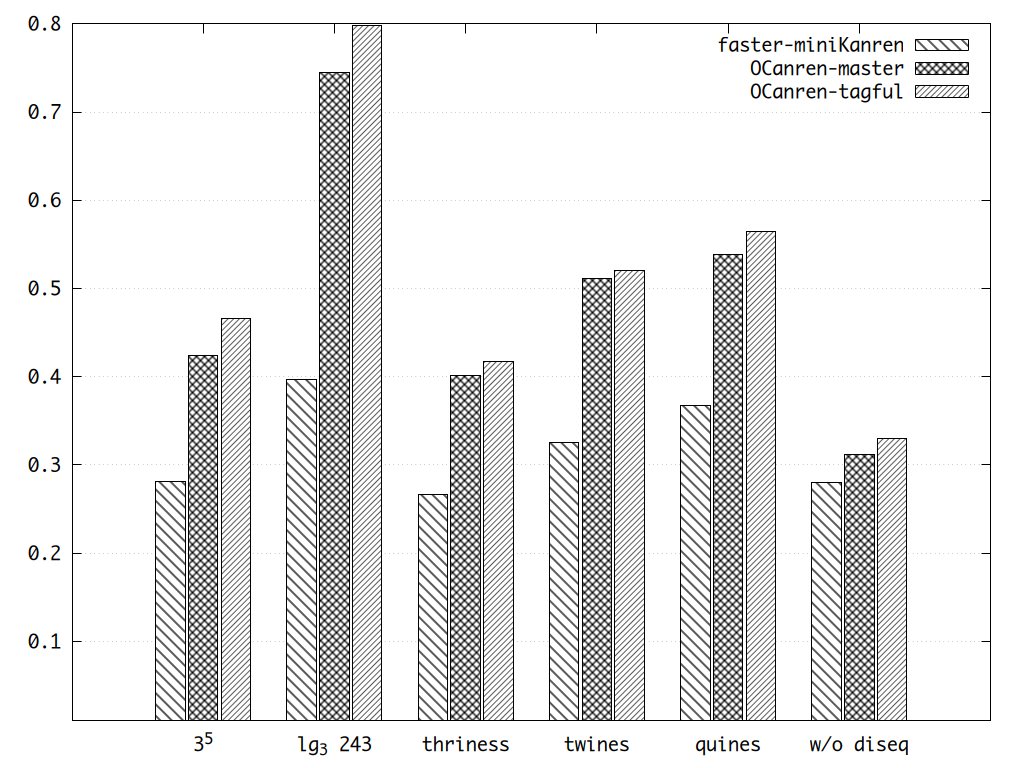
\includegraphics[scale=0.8]{graph.png}
\caption{Результаты оценки производительности}
\label{eval}
\end{figure}

\FloatBarrier

Для набора тестов были выбраны следующие задачи:
%For the set of benchmarks we took the following problems:

\begin{itemize}
\item \textbf{pow, logo}~--- реляционное возведение в степень и логарифмирование~\cite{KiselyovArithm} чисел в двоичном представлении.
Конкретно выбраны $3^5=243$ и $log_3 243=5$.
%and logarithm for integers in binary form. The concrete tests relationally computed
%$3^5$ (which is 243) and $log_3 243$ (which is, conversely, 5). The implementaion was adopted from~\cite{KiselyovArithm}.
\item \textbf{quines, twines, trines}~--- программы, вычисляющиеся в себя, использованные для тестирования реляционных интерпретаторов~\cite{Untagged}.
Конкретно тесты вычисляю первые 100, 15 и 2 ответа(ов) для соответствующих задач.
%\item \textbf{quines, twines, trines}~--- self/co-evaluating program synthesis problems from~\cite{Untagged}. The
%concrete tests took the first 100, 15 and 2 answers for these problems respectively.
\end{itemize}

%Since the last bundle of benchmarks uses disequality constraints (and, hence, $\mu$Kanren is ruled out) we
%split all benchmarks into two sets.

Вычисления производились на компьютере с процессором Intel Core i7-4790K CPU @ 4.00GHz и 16GB памяти.
Для OCanren использовался компилятор \texttt{OCaml-4.14.2+flambda}, для faster-miniKanren~--- Chez~Scheme~9.5.8.
Все бенчмарки компилировались в нативный код и вычислялось среднее время за 40 испытаний.
Результаты представлены на рисунке~\ref{eval}.
Репозиторий с кодом и инструкции по воспроизведению эксперимента доступны на GitHub\footnote{\url{https://github.com/Kakadu/ocanren-perf/tree/ispras-paper2025}}.
%All benchmarks were executed in the natively compiled mode ten times, then average user time was taken. The results of the evaluation
%are shown on Figure~\ref{eval}. The whole evaluation repository with all scripts and detailed description is accessible
%from \lstinline|GitHub|\footnote{\url{https://github.com/Kakadu/ocanren-perf/tree/ispras-paper2025}}.

Наблюдения показывают, что важность нетегированного представления варьируется от задачи.
В зависимости от видов термов, участвующих в унификации, прирост производительности будет разниться.
Действительно, если термы являются копиями друг друга, то унификации нужно совершить полный обход термов. Если же термы не равны, то унификация может завершиться раньше, без полного обхода термов.
%The first conclusion, which is rather easy to derive from the results, is that the tagless approach indeed matters. Our initial
%implementation did not show essential speedup in comparison even with $\mu$Kanren (and was even \emph{slower} on the logarithm
%and permutations benchmarks). The situation was improved drastically, however, when we switched to the tagless version.

Также стоит отметить, что реализация на OCaml отстаёт по сравнению с реализацией для Chez Scheme. Вероятно, это связано с особенностями хранения данных~\cite{BIBOP94} в реализации компилятора. Детальное исследование различий сред исполнения OCaml и Scheme оставлено на будущее.
%Yet, in comparison with faster-miniKanren, our implementation is still lagging behind. We can conclude that the optimizNfr;tations
%used in the Scheme/Racket version, have a different impact in the OCaml case; we save this problem for future research.


\section{Conclusion and future work}

We presented an approach for pattern matching implementation synthesis using relational programming. Currently, it demonstrates a good performance only
on a very small problems. The performance can be improved by searching for new ways to prune the search space and by speeding up the implementation of
relations and structural constraints. Also it could be interesting to integrate structural constraints more closely into \textsc{OCanren}'s core.
Discovering an optimal order of samples and reducing the complete set of samples is another direction for research.

The language of intermediate representation can be altered, too. It is interesting to add to an intermediate language so-called \emph{exit nodes}
described in~\cite{maranget2001}. The straightforward implementation of them might require nominal unification, but we are not aware of any
\textsc{miniKanren} implementation in which both disequality constraints and nominal unification~\cite{alphaKanren} coexist nicely.

At the moment we support only simple pattern matching without any extensions. It looks technically easy to extend our approach with
non-linear and disjunctive patterns. It will, however, increase the search space and might require more optimizations.





%%
%% The acknowledgments section is defined using the "acks" environment
%% (and NOT an unnumbered section). This ensures the proper
%% identification of the section in the article metadata, and the
%% consistent spelling of the heading.
\begin{acks}
To Robert, for the bagels and explaining CMYK and color spaces.
\end{acks}

%%
%% The next two lines define the bibliography style to be used, and
%% the bibliography file.
\bibliographystyle{ACM-Reference-Format}
\bibliography{ocanren}


%%
%% If your work has an appendix, this is the place to put it.
%\appendix


\end{document}
\endinput
%%
%% End of file `sample-acmsmall.tex'.
